% Тут используется класс, установленный на сервере Papeeria. На случай, если
% текст понадобится редактировать где-то в другом месте, рядом лежит файл matmex-diploma-custom.cls
% который в момент своего создания был идентичен классу, установленному на сервере.
% Для того, чтобы им воспользоваться, замените matmex-diploma на matmex-diploma-custom
% Если вы работаете исключительно в Papeeria то мы настоятельно рекомендуем пользоваться
% классом matmex-diploma, поскольку он будет автоматически обновляться по мере внесения корректив
%

% По умолчанию используется шрифт 14 размера. Если нужен 12-й шрифт, уберите опцию [14pt]
%\documentclass[14pt]{matmex-diploma}
\documentclass[14pt]{matmex-diploma-custom}
% таблицы
\usepackage{multirow}
\usepackage{pdflscape}
\usepackage{graphicx}

\usepackage{svg}

\usepackage{fontspec}
\usepackage{polyglossia}
\usepackage{amsmath}
\usepackage{amsfonts}
\usepackage{amssymb}

% пакеты из презентации
\usepackage{algpseudocode}
\usepackage{algorithm}
\usepackage{algorithmicx}
\usepackage{pdfpages}

\usepackage{subcaption}
\usepackage{geometry}
\usepackage{amsfonts,latexsym}
\usepackage{amsthm}
\usepackage{amssymb}
\usepackage[utf8]{inputenc} % Кодировка
\usepackage{mathtools}
\usepackage{hyperref}
\usepackage{tikz}
\usepackage{dsfont}
\usepackage{multicol}
\usetikzlibrary{fit,calc,automata,positioning}

\theoremstyle{definition}
\newtheorem{rudefinition}{Определение}[section]
\newtheorem{ruexample}{Пример}[section]
\newtheorem{example}{Example}[section]
\newtheorem{theorem}{Theorem}[section]
\newtheorem{proposition}[theorem]{Proposition}
\newtheorem{lemma}[theorem]{Lemma}
\newtheorem{corollary}[theorem]{Corollary}
\newtheorem{conjecture}[theorem]{Conjecture}
\newtheorem{note}[theorem]{Утверждение}

%code highlight
% \usepackage{listings}
\usepackage{listings, listings-rust}
\usepackage{lipsum}
\usepackage{xcolor}

\usepackage{tikz}
\usetikzlibrary{decorations.pathreplacing,calc,shapes,positioning}

\newcommand\tbox[1]{\tikz[overlay]\node[inner sep=2pt, draw=red, ultra thick, anchor=text, rectangle] {#1};\phantom{#1}}

\definecolor{codegreen}{rgb}{0,0.6,0}
\definecolor{codegray}{rgb}{0.5,0.5,0.5}
\definecolor{codepurple}{rgb}{0.58,0,0.82}
\definecolor{backcolour}{rgb}{1,1,1}
 
\lstdefinestyle{mystyle}{
    backgroundcolor=\color{backcolour},   
    commentstyle=\color{codegreen},
    keywordstyle=\color{magenta},
    numberstyle=\color{codegray},
    stringstyle=\color{codepurple},
    basicstyle=\ttfamily\small,
    breakatwhitespace=false,         
    breaklines=true,                 
    captionpos=b,                    
    keepspaces=true,                 
    numbers=left,                    
    numbersep=5pt,                  
    showspaces=false,                
    showstringspaces=false,
    showtabs=false,                  
    tabsize=2
    % xleftmargin=.2\textwidth,
    % xrightmargin=.2\textwidth
}
 
\lstset{style=mystyle}

\lstnewenvironment{code}[1][]%
{
   \noindent
   \minipage{\linewidth} 
   \vspace{0.5\baselineskip}
   \lstset{basicstyle=\ttfamily\footnotesize,frame=single,#1}}
{\endminipage}

\begin{document}
\filltitle{ru}{
    %% Актуально только для курсовых/практик. ВКР защищаются не на кафедре а в ГЭК по направлению, 
    %%   и к моменту защиты вы будете уже не в группе.
    chair              = {Кафедра, на которой работает научник},
    group              = {19.Б11-мм},
    %
    %% Макрос filltitle ненавидит пустые строки, поэтому обязателен хотя бы символ комментария на строке
    %% Актуально всем.
    title              = {Реализация и экспериментальное исследование GLL-парсера, основанного на рекурсивном автомате},
    % 
    %% Здесь указывается тип работы. Возможные значения:
    %%   coursework - отчёт по курсовой работе;
    %%   practice - отчёт по учебной практике;
    %%   prediploma - отчёт по преддипломной практике;
    %%   master - ВКР магистра;
    %%   bachelor - ВКР бакалавра.
    type               = {bachelor},
    %
    %% Здесь указывается вид работы. От вида работы зависят критерии оценивания.
    %%   solution - <<Решение>>. Обучающемуся поручили найти способ решения проблемы в области разработки программного обеспечения или теоретической информатики с учётом набора ограничений.
    %%   experiment - <<Эксперимент>>. Обучающемуся поручили изучить возможности, достоинства и недостатки новой технологии, платформы, языка и т. д. на примере какой-то задачи.
    %%   production - <<Производственное задание>>. Автору поручили реализовать потенциально полезное программное обеспечение.
    %%   comparison - <<Сравнение>>. Обучающемуся поручили сравнить несколько существующих продуктов и/или подходов.
    %%   theoretical - <<Теоретическое исследование>>. Автору поручили доказать какое-то утверждение, исследовать свойства алгоритма и т.п., при этом не требуя написания кода.
    kind               = {experiment},
    %
    author             = {АБЗАЛОВ Вадим Игоревич},
    % 
    %% Актуально только для ВКР. Указывается код и название направления подготовки. Типичные примеры:
    %%   02.03.03 <<Математическое обеспечение и администрирование информационных систем>>
    %%   02.04.03 <<Математическое обеспечение и администрирование информационных систем>>
    %%   09.03.04 <<Программная инженерия>>
    %%   09.04.04 <<Программная инженерия>>
    %% Те, что с 03 в середине --- бакалавриат, с 04 --- магистратура.
    specialty          = {09.03.04 <<Программная инженерия>>},
    % 
    %% Актуально только для ВКР. Указывается шифр и название образовательной программы. Типичные примеры:
    %%   СВ.5006.2017 <<Математическое обеспечение и администрирование информационных систем>>
    %%   СВ.5162.2020 <<Технологии программирования>>
    %%   СВ.5080.2017 <<Программная инженерия>>
    %%   ВМ.5665.2019 <<Математическое обеспечение и администрирование информационных систем>>
    %%   ВМ.5666.2019 <<Программная инженерия>>
    %% Шифр и название программы можно посмотреть в учебном плане, по которому вы учитесь. 
    %% СВ.* --- бакалавриат, ВМ.* --- магистратура. В конце --- год поступления (не обязательно ваш, если вы были в академе/вылетали).
    programme          = {СВ.5080.2019 <<Программная инженерия>>},
    % 
    %% Актуально только для ВКР, только для матобеса и только 2017-2018 годов поступления. Указывается профиль подготовки, на котором вы учитесь.
    %% Названия профилей можно найти в учебном плане в списке дисциплин по выбору. На каком именно вы, вам должны были сказать после второго курса (можно уточнить в студотделе).
    %% Вот возможные вариканты:
    %%   Математические основы информатики
    %%   Информационные системы и базы данных
    %%   Параллельное программирование
    %%   Системное программирование
    %%   Технология программирования
    %%   Администрирование информационных систем
    %%   Реинжиниринг программного обеспечения
    % profile            = {Системное программирование},
    % 
    %% Актуально всем.
    %supervisorPosition = {проф. каф. СП, д.ф.-м.н., проф.}, % Терехов А.Н.
    supervisorPosition = {доцент кафедры информатики, кандидат физико-математических наук}, % Григорьев С.В.
    supervisor         = {Григорьев С.В.},  
    % 
    %% Актуально только для практик и курсовых. Если консультанта нет, закомментировать или удалить вовсе.
    % consultantPosition = {должность ООО <<Место работы>> степень},
    % consultant         = {К.К. Консультант},
    %
    %% Актуально только для ВКР.
    reviewerPosition   = {академический консультант, кандидат физико-математических наук},
    reviewer           = {Азимов Р.Ш.},
}

\filltitle{en}{
    chair              = {Software Engineering},
    group              = {19.B11-mm},
    title              = {Implementation and experimental study of the GLL-parser based on a recursive automaton},
    type               = {bachelor},
    author             = {Vadim Abzalov},
    % 
    %% Possible choices:
    %%   02.03.03 <<Software and Administration of Information Systems>>
    %%   02.04.03 <<Software and Administration of Information Systems>>
    %%   09.03.04 <<Software Engineering>>
    %%   09.04.04 <<Software Engineering>>
    %% Те, что с 03 в середине --- бакалавриат, с 04 --- магистратура.
    specialty          = {09.03.04 <<Software Engineering>>},
    % 
    %% Possible choices:
    %%   СВ.5006.2017 <<Software and Administration of Information Systems>>
    %%   СВ.5162.2020 <<Programming Technologies>>
    %%   СВ.5080.2017 <<Software Engineering>>
    %%   ВМ.5665.2019 <<Software and Administration of Information Systems>>
    %%   ВМ.5666.2019 <<Software Engineering>>
    programme          = {СВ.5080.2018 <<Software Engineering>>},
    % 
    %% Possible choices:
    %%   Mathematical Foundations of Informatics
    %%   Information Systems and Databases
    %%   Parallel Programming
    %%   System Programming
    %%   Programming Technology
    %%   Information Systems Administration
    %%   Software Reengineering
    % profile            = {Software Engineering},
    % 
    %% Note that common title translations are:
    %%   кандидат наук --- C.Sc. (NOT Ph.D.)
    %%   доктор ... наук --- Sc.D.
    %%   доцент --- docent (NOT assistant/associate prof.)
    %%   профессор --- prof.
    supervisorPosition = {C.Sc., docent},
    supervisor         = {Semyon Grigorev},
    % 
    % consultantPosition = {position at ``Company'', degree if present},
    % consultant         = {C.C. Consultant},
    %
    reviewerPosition   = {academic advisor, C.Sc. of Physics and Mathematics},
    reviewer           = {Rustam Azimov},
}
% Год, город, название университета и факультета предопределены,
% но можно и поменять.
% Если англоязычная титульная страница не нужна, то ее можно просто удалить.

\newcommand\todo[1]{{\color{violet}#1}}
\newcommand\db[1]{{\color{red}#1}}
\newcommand\question[1]{{\color{cyan}#1}}

\maketitle
\tableofcontents
% У введения нет номера главы
\section{Introduction}

% Commented references
% CuSha~\cite{10.1145/2600212.2600227}
% MapGraph~\cite{10.1145/2621934.2621936/MapGraph}
% Medusa~\cite{6497047/Medusa}
% Gunrock~\cite{7967137}

Scalable high-performance graph analysis is a challenge.
CuSha~\cite{10.1145/2600212.2600227} and Gunrock~\cite{7967137} show that the utilization of GPUs can improve the performance of graph analysis. But the low flexibility and high complexity of API are problems of these solutions. 
A linear algebra based model, formalized in GraphBLAS~\cite{7761646}, provides a user-friendly API. 
While the reference CPU-based implementation for this API, SuiteSparse~\cite{10.1145/3322125}, demonstrates good performance on real-world tasks, GPU-based implementation is challenging due to required operations generalization, data sparsity, and hardware programming complexity. 
Such well-known libraries as cuSPARSE, clSPARSE, bhSPARSE cannot be reused, since almost all of them are specified for operations over floats. 
GraphBLAST~\cite{yang2019graphblast} and GBTL~\cite{7529957} show promising GPU performance of GraphBLAS-based graph analysis solutions. 
But these solutions are not portable because they are based on Nvidia Cuda. 
Portable solution is a challenge due to intricate GPU programming. 
To address this problem, we developed the GraphBLAS-inspired \textit{Spla\footnote{Source code and project page: \url{github.com/SparseLinearAlgebra/spla}}} library, which features portable OpenCL-based acceleration and shows performance comparable with GraphBLAST, achieving speedup of up to 36 times.
\section{Постановка задачи}\label{ps}
Целью данной работы является реализация и экспериментальное исследование производительности GLL-парсера, основанного на рекурсивном автомате.

Для достижения данной цели были поставлены следующие задачи.

\begin{itemize}
    \item Реализация классического алгоритма GLL.
    \item Модификация алгоритма GLL для поддержки представления грамматики в виде рекурсивного автомата.
    \item Расширение модифицированного алгоритма GLL на входные данные в виде графа.
    \item Проведение экспериментального исследования и сравнение с существующими решениями.
\end{itemize}
\section{Обзор}

Данный раздел содержит ряд базовых определений из теории формальных языков, а далее --- краткое описание алгоритмов поиска путей с контекстно-свободными ограничениями.

\subsection{Базовые определения из теории формальных языков}
Введем базовые определения из теории формальных языков, которые будут использоваться в дальнейшем.

\begin{rudefinition}
     \emph{Контекстно-свободная грамматика} --- это четверка $\mathbb{G} = \langle N, \Sigma, P, S \rangle $, где
     \begin{itemize}
          \item $N$ --- конечное множество нетерминальных символов;
          \item $\Sigma$ --- конечное множество терминальных символов, $ \Sigma \cap N = \varnothing $;
          \item $P$ --- конечное множество правил или продукций вида $A \rightarrow \alpha$, где $A \in N$ и $\alpha  \in \{ \Sigma \cup N \}^*$ или $\alpha = \varepsilon$;
          \item $S \in N$ --- стартовый нетерминал.
     \end{itemize}
\end{rudefinition}

Важную роль в данной работе играет понятие \emph{выводимости слова в контекстно-свободной грамматике}.
Необходимые определения приведены ниже.

\begin{rudefinition}
    \emph{Шаг вывода в контекстно-свободной грамматике} $\mathbb{G} = \langle N, \Sigma, P, S \rangle$ --- это переход $\gamma A \beta \Rightarrow \gamma \alpha \beta$, где $\gamma, \beta \in \{ \Sigma \cup N \}^*$ и $(A \rightarrow \alpha) \in P$
\end{rudefinition}

\begin{rudefinition}
    Слово $w \in \Sigma^*$ \emph{выводимо в контекстно-свободной грамматике} $\mathbb{G} = \langle N, \Sigma, P, S \rangle$, если существует последовательность шагов вывода в грамматике $\mathbb{G}$: $S \Rightarrow \beta_0 \Rightarrow \beta_1 \Rightarrow \dots \Rightarrow \beta_{n - 1} \Rightarrow w$.
    Будем обозначать это как $S \xRightarrow[]{*} w$.
\end{rudefinition}

\begin{rudefinition}
     \emph{Язык, задаваемый контекстно-свободной грамматикой} $\mathbb{G} = \langle N, \Sigma, P, S \rangle$ --- это множество слов, выводимых в грамматике $$L(\mathbb{G}) = \{ w \in \Sigma^* | S \xRightarrow[]{*} w\}$$
\end{rudefinition}

Наравне с контекстно-свободными грамматиками в этой работе также используются рекурсивные автоматы, поэтому введем соответствующие определения.

\begin{rudefinition}
    \emph{Детерминированный конечный автомат} --- это пятерка $\langle Q, \Sigma, \sigma, Q_{0}, Q_{F}\rangle$:
    \begin{itemize}
        \item $Q$ --- конечное множество состояний;
        \item $\Sigma$ --- конечное множество входных символов;
        \item $\sigma ~:~ Q \times \Sigma \rightarrow Q$ --- функция переходов, аргументами которой являются текущее состояние и входной символ, а значением --- новое состояние;
        \item $Q_{0}$ --- начальное состояние, $Q_{0} \in Q$;
        \item $Q_{F}$ --- множество допускающих состояний, $Q_{F} \subseteq Q$.
    \end{itemize}
\end{rudefinition}

Рекурсивный автомат является обобщением детерминированного конечного автомата и позволяет задавать те же языки, что задаются контекстно-свободными грамматиками.

\begin{rudefinition}
    \emph{Рекурсивный автомат} --- это семерка $$\mathbb{A} = \langle Q, \Sigma, N, \sigma, Q_{S}, Q_{F}, S\rangle$$
    \begin{itemize}
        \item $Q$ --- конечное множество состояний, каждое состояние помечено нетерминалом;
        \item $N$ --- конечное множество нетерминальных символов;
        \item $\Sigma$ --- конечное множество терминальных символов, $\Sigma \cap N = \varnothing$;
        \item $\sigma ~:~ Q \times (\Sigma \cup N) \rightarrow Q$ --- функция переходов, аргументами которой являются текущее состояние и символ из $\Sigma \cup N$, а значением --- новое состояние;
        \item $Q_{S}$ --- множество начальных состояний, $Q_{S} \subseteq Q$;
        \item $Q_{F}$ --- множество допускающих состояний, $Q_{F} \subseteq Q$;
        \item $S$ --- стартовый нетерминал, $S \in N$.
    \end{itemize}
\end{rudefinition}

Рекурсивный автомат отличается от детерминированного конечного автомата тем, что:
\begin{itemize}
    \item вместо одного конечного автомата, рекурсивный автомат может состоять из нескольких конечных автоматов, каждый из который помечен своим уникальным нетерминалом;
    \item переходы по терминальным символам осуществляются также, как и в детерминированном конечном автомате, однако переходы по нетерминальным символам осуществляются тогда и только тогда, когда рекурсивный спуск в конечный автомат, стартовое состояние которого помечено нетерминальным символом перехода, завершается в допускающем состоянии соответствующего автомата.
\end{itemize}

\begin{ruexample}
    Рассмотрим язык $\mathbb{L}_0 = \{a^n b^n ~|~ n \in \mathbb{N}\}$.
    Язык $\mathbb{L}_0$ представляет собой конкатенацию $n$ букв "$a$" и $n$ букв "$b$", где $n$ --- натуральное число.
\end{ruexample}
Этот язык может быть задан с помощью контекстно-свободной грамматики.

\begin{ruexample}
    \emph{Контекстно-свободная грамматика $\mathbb{G}_0 $, задающая язык $\mathbb{L}_0$}.
    $$S \rightarrow a S b$$
    $$S \rightarrow a b$$
\end{ruexample}

\begin{ruexample}
    \emph{Пример вывода слова $aaabbb \in \mathbb{L}_0$ в грамматике $\mathbb{G}_0$}.
    $$S \Rightarrow a S b \Rightarrow a a S b b \Rightarrow a a a b b b$$
\end{ruexample}

Этот же язык возможно задать с помощью рекурсивного автомата.

\begin{ruexample}
    \emph{Рекурсивный автомат $\mathbb{A}_0$, задающий язык $\mathbb{L}_0$}.

    \begin{align}
    \label{rsm0}
        \begin{tikzpicture}[node distance=2.5cm,shorten >=1pt,on grid,auto]
           \node[state, initial] (q_0)   {$0 \{S\}$};
           \node[state] (q_1) [right=of q_0] {$1 \{S\}$};
           \node[state] (q_2) [right=of q_1] {$2 \{S\}$};
           \node[state, accepting] (q_3) [right=of q_2] {$3 \{S\}$};
            \path[->]
            (q_0) edge  node {a} (q_1)
            (q_1) edge  node {S} (q_2)
            (q_2) edge  node {b} (q_3)
            (q_1) edge[bend left, above]  node {b} (q_3);
        \end{tikzpicture}
    \end{align}
    
\end{ruexample}

\begin{ruexample}
    \emph{Пример вывода слова $aaabbb \in \mathbb{L}_0$ в рекурсивном автомате $\mathbb{A}_0$}.
    $$0 \xRightarrow[]{a} 1 \xRightarrow[\text{rec}\downarrow]{S} 0 \xRightarrow[]{a} 1 \xRightarrow[\text{rec}\downarrow]{S} 0 \xRightarrow[]{a} 1 \xRightarrow[]{b} 3 \xRightarrow[\text{rec}\uparrow]{S} 2 \xRightarrow[]{b} 3 \xRightarrow[\text{rec}\uparrow]{S} 2 \xRightarrow[]{b} 3$$

    Здесь $\text{rec}\downarrow$ обозначает рекурсивный спуск в рекурсивном автомате, а $\text{rec}\uparrow$ возврат из рекурсивного спуска.
\end{ruexample}


\subsection{Базовые определения из теории графов}

Введем базовые определения из теории графов, которые будут использоваться в дальнейшем.

\begin{rudefinition} \emph{Помеченный ориентированный граф} --- это тройка $\mathbb{D} = \langle V, E, T \rangle$, где
\begin{itemize}
    \item $V$ --- конечное множество вершин, не умаляя общности пронумеруем вершины натуральными числами от $0$ до $|V|-1$;
    \item $T$ --- конечное множество меток на ребрах;
    \item $E \subseteq V \times T \times V$ --- конечное множество ребер.
\end{itemize}
\end{rudefinition}

\begin{rudefinition}
 \emph{Путь $\pi$ в графе} $\mathbb{D} = \langle V, E, T \rangle$ --- это конечная последовательность ребер $(e_0, e_1, ..., e_{n-1})$, где $\forall~ j,~ 0 \leq j \leq n - 1: e_j=(v_j,t_j,v_{j+1}) \in E$.
Определим множество всех путей в графе $\mathbb{D}$ как $\pi(\mathbb{D})$.
\end{rudefinition}

\begin{rudefinition}
    \emph{Слово, соответствующее пути} $\pi = (e_0, e_1, ..., e_{n-1})$, определим как последовательную конкатенацию меток ребер пути $l(\pi) = t_0 t_1 \dots t_{n - 1}$.
\end{rudefinition}

\subsection{Задачи поиска путей с контекстно-свободными ограничениями}
Теперь мы можем приступить к формальным определениям задач поиска путей с контекстно-свободными ограничениями.

Пусть даны:
\begin{itemize}
      \item контекстно-свободная грамматика $\mathbb{G} = \langle N, \Sigma, P, S \rangle$;
      \item помеченный ориентированный граф $\mathbb{D} = \langle V, E, T \rangle$;
      \item  множество стартовых вершин $V_S \subseteq V$ и множество финальных вершин \mbox {$V_F \subseteq V$}.
\end{itemize}

В введенных обозначениях могут быть сформулированы cледующие задачи.

\begin{itemize}
    \item \textbf{Задача поиска путей в графе с контекстно-свободными ограничениями} состоит в нахождении всех путей в графе таких что $l(\pi) \in L(\mathbb{G})$ и $v_0 \in V_S, ~v_n \in V_F$.
    \item \textbf{Задача поиска достижимостей в графе с контекстно-сво-бодными ограничениями} заключается в поиске множества пар вершин, для которых существует такой путь с началом и концом в этих вершинах, что слово, составленное из меток рёбер пути, принадлежит заданному языку: $\{(v_i, v_j ) ~|~ \exists ~l(\pi): ~l(\pi) \in L(\mathbb{G})$ и $v_0 \in V_S, ~v_n \in V_F\}$.
\end{itemize}

\subsection{Обобщенный LL алгоритм}
Одной из наиболее популярных техник синтаксического разбора является LL(k)-парсер, который представляет собой алгоритм нисходящего анализа с предпросмотром. 
Это означает, что решение о том, какая из продукций контекстно-свободной грамматики должна быть применена, базируется на предпросмотре $k$ следующих от текущего символов.
Для выбора правильной продукции поддерживается специальная таблица, в которой хранится информация для разбора текущего символа.
Однако, этот алгоритм может быть применен лишь к небольшому подмножеству контекстно-свободных грамматик.
Например, данный алгоритм неприменим к неоднозначным грамматикам или грамматикам с непосредственной левой рекурсией.

Алгоритмы нисходящего анализа относительно проще реализовывать и отлаживать, чем алгоритмы восходящего анализа, так как они полностью соотносятся со структурой грамматики.
По этой причине для того, чтобы поддержать весь класс контекстно-свободных грамматик, был предложен обобщенный вариант LL(k) алгоритма --- GLL (Generalized LL)~\cite{intro}. 
В случае LL(k) алгоритма может возникнуть такая ситуация, что невозможно определить, какая продукция должна быть выбрана в текущем состоянии синтаксического разбора.
Для решения данной проблемы в GLL вместо выбора одной продукции выбираются все допустимые продукции.
Такой подход позволяет во время работы алгоритма рассмотреть все возможные переходы из одного состояния разбора в другое.

Процесс работы GLL можно рассматривать как процесс обхода грамматики, управляемый входной строкой.
В каждый момент времени работы алгоритма GLL поддерживается дескриптор, состоящий из следующих объектов: $\langle A \rightarrow \alpha, c_{\alpha} \rangle$ --- \emph{позиция в грамматике}, $c_{i}$ --- \emph{позиция во входной строке}, $c_{u}$ --- \emph{текущая вершина GSS}, $c_{N}$ --- \emph{текущая вершина SPPF}.

\begin{rudefinition}
    \emph{Позиция в грамматике} --- это пара $\langle A \rightarrow \alpha, c_{\alpha} \rangle$, содержащая текущую продукцию в грамматике $A \rightarrow \alpha$ и индекс текущего символа в продукции соответственно.
    Наряду с обозначением $\langle A \rightarrow \alpha, c_{\alpha} \rangle$ примем обозначение $A \rightarrow \alpha \cdot X \beta$, где $c_{\alpha}$ соответствует индексу символа $X$, который может быть как терминальным, так и нетерминальным.
\end{rudefinition}

\begin{rudefinition}
    \emph{Позиция во входной строке} $c_{i}$ --- это индекс текущего символа во входной строке.
\end{rudefinition}

\begin{rudefinition}
    \emph{GSS} или \emph{графо-структурированный стек} --- граф, предназначенный для замены стека из LL(k)-парсера, вершины которого представляют пары $\langle \mathbb{L}, c_{i} \rangle$, что соответствует позиции в грамматике и позиции во входной строке на момент создания вершины, то есть некоторому состоянию разбора, а ребра обозначают рекурсивные переходы по грамматике и помечены соответствующими SPPF вершинами.
\end{rudefinition}

\begin{rudefinition}
    \emph{SPPF} --- сжатое представление леса разбора, которое содержит в себе все деревья вывода входной строки. 
\end{rudefinition}

Четверка $\langle \langle A \rightarrow \alpha, c_{\alpha} \rangle, c_{u}, c_{i}, c_{N} \rangle$ --- называется дескриптором.
В ходе работы GLL алгоритма поддерживается два множества:
\begin{itemize}
    \item $\mathbb{R}$ --- множество всех еще необработанных дескрипторов, представленное в виде очереди;
    \item $\mathbb{U}$ --- множество всех уже обработанных дескрипторов.
\end{itemize}
Изначально $\mathbb{R} = \{ \langle \langle S, 0 \rangle, c_{u}^{\varnothing}, 0, c_{N}^{\varnothing} \rangle \}$ и $\mathbb{U} = \varnothing$,
где $c_{u}^{\varnothing}$ --- специальная стартовая GSS вершина, $c_{N}^{\varnothing}$ --- пустое SPPF дерево.
Когда GLL алгоритм встречает терминальный символ на текущей позиции в грамматике $\langle A \rightarrow \alpha, c_{\alpha} \rangle$, если он совпадает с текущим символом входной строки, то в $\mathbb{R}$ добавляется дескриптор $\langle \langle A \rightarrow \alpha, c_{\alpha} + 1 \rangle, c_{u}, c_{i} + 1, c_{N}^{new} \rangle$, где $c_{N}^{new}$ является SPPF деревом разбора подстроки $0 \dots c_{i} + 1$, иначе, если символ на текущей позиции в грамматике не совпадает с текущим символом входной строки, то осуществляеся переход к следующему дескриптору в очереди $\mathbb{R}$.
Когда GLL алгоритм встречает нетерминальный символ на текущей позиции в грамматике $A \rightarrow \alpha \cdot X \beta$, создается вершина GSS $c_{u}^{new}$, содержащая текущее состояние разбора, и для каждой продукции $(X \rightarrow \gamma) \in P$ в $\mathbb{R}$ добавляются дескрипторы вида $\langle \langle X \rightarrow \gamma, 0 \rangle, c_{u}^{new}, c_{i}, c_{N}^{\varnothing} \rangle$, которых еще нет в $\mathbb{U}$.
GLL алгоритм завершается тогда, когда $\mathbb{R} = \varnothing$.

\subsection{Алгоритм выполнения контекстно-свободных запросов, базирующийся на GLL}
Как было сказано выше, алгоритмы на основе нисходящего анализа могут быть использованы для решения задачи поиска путей с контекстно-свободными ограничениями.
Более того, GLL алгоритм довольно естественным путем обобщается на входные данные в виде графов~\cite{GLL2}: вместо того, чтобы позициями входа считать индексы линейного входа, теперь будем считать ими вершины графа. 

Для сохранения корректности работы алгоритма вносятся следующие изменения. 

\begin{itemize}
\item Запрос теперь представляет собой тройку: множество стартовых вершин, множество финальных вершин и грамматику.
\item \emph{Позиция во входной строке} заменяется на вершину графа.
\item Начальное множество дескрипторов инициализируется дескрипторами, каждый из которых содержит стартовую вершину запроса.
\item На шаге перехода в грамматике обрабатываются все переходы по исходящим ребрам текущей вершины графа;
\item Если разбор завершен, необходимо проверить принадлежность вершины, на которой алгоритм остановился, к множеству финальных вершин графа.
\end{itemize}

Так же, как и в случае стандартного GLL алгоритма, данная модификация способна обрабатывать произвольные контекстно-свободные грамматики. 
\section{Реализация алгоритма}\label{ps}

Прежде чем приступать к реализации модификации приведем пример, иллюстрирующий мотивацию предлагаемой модификации.

\subsection{Мотивация}

В классическом GLL алгоритме дескриптор содержит в себе \emph{позицию в грамматике} --- текущую обрабатываемую продукцию и позицию в этой продукции, обозначающаю какие элементы продукции уже были обработаны.
Таким образом для каждой продукции грамматики в GLL алгоритме неизбежно создается как минимум столько дескрипторов, сколько в этой продукции символов.

\begin{ruexample}
    Рассмотрим простой язык, состоящий из нуля и более повторений буквы $a$: $\mathbb{L}_1 = \{a\}^*$.
\end{ruexample}

\begin{ruexample}
    Контекстно-свободная грамматика $\mathbb{G}_1$, задающая язык $\mathbb{L}_1$.
    $$S \longrightarrow a S$$
    $$S \longrightarrow \varepsilon$$
\end{ruexample}
Для такой грамматики в ходе работы GLL алгоритма будет создано целых четыре \emph{позиции в грамматике}, и, соответственно, не меньше четырех дескрипторов.

Однако этот же язык можно выразить с помощью рекурсивного автомата всего на одном состоянии и одном переходе, а для такого автомата количество созданных GLL алгоритмом дескрипторов будет гораздо меньше.

\begin{ruexample}
    Рекурсивный автомат $\mathbb{A}_1$, задающий язык $\mathbb{L}_1$.

    \begin{align}
    \label{input2}
        \begin{tikzpicture}[node distance=2.5cm,shorten >=1pt,on grid,auto]
           \node[state, initial, accepting] (q_0)   {$0 \{S\}$};
            \path[->]
            (q_0) edge[loop, above]  node {a} (q_0);
        \end{tikzpicture}
    \end{align}

\end{ruexample}

Так как производительность GLL алгоритма напрямую зависит от количества создаваемых дескрипторов, возникает предположение о модификации классического GLL алгоритма путем замены контекстно-свободной грамматики на рекурсивный автомат.

\subsection{Особенности реализации} 

Предлагаемая в данной работе модификация GLL алгоритма основана на замене в дескрипторе \emph{позиции в грамматике} на состояние рекурсивного автомата, то есть в четверке $\langle \langle A \rightarrow \alpha, c_{\alpha} \rangle, c_{u}, c_{i}, c_{N} \rangle$ пара $\langle A \rightarrow \alpha, c_{\alpha} \rangle$ заменяется на $c_{R}$ --- текущее состояние рекурсивного автомата.
Соответственно переход в контекстно-свободной грамматике заменяется на переход в рекурсивном автомате.

Данная модификация, как и классический GLL алгоритм, может быть обобщена на графы --- на шаге перехода в рекурсивном автомате обрабатываются все переходы из текущего состояния рекурсивного автомата по всем исходящим ребрам текущей вершины графа.

Одной из недавних удачных реализаций GLL алгоритма является библиотека GLL4Graph\footnote{Github репозиторий библиотеки: \url{https://github.com/FormalLanguageConstrainedPathQuerying/GLL4Graph}. Accessed: 05/04/2023}, написанная на языке программирования Java.
Это означает, что виртуальная машина Java, она же JVM, является подходящей для эффективной реализации такого рода алгоритмов.
С другой стороны, опираясь на то, что данная работа является возможной основой для дальнейших расширений и оптимизаций, не менее важным было не только разработать оптимальную для этих целей архитектуру, но и сделать сам код реализации максимально лаконичным и понятным.
По сравнению с языком программирования Java, программа, написанная на языке программирования Kotlin имеет более читаемый и структурно точный код, что облегчает не только ее понимание, но и дальнейшую поддержку. 
Поэтому в качестве языка программирования для реализации модификации GLL алгоритма был выбран язык Kotlin.

\subsection{Архитектура}

Прежде, чем приступать к модификации GLL алгоритма, необходимо реализовать его классический вариант.
В связи с этим возникает вопрос о разработке подходящей архитектуры для проекта в целом.
Поэтому были разработаны следующие требования.
\begin{itemize}
    \item Для удобства модификации и дальнейшей поддержки кода каждая реализация GLL алгоритма должна находиться в отдельном модуле и не зависеть от других реализаций.
    \item Кроме GLL алгоритмов, с входными данными, представленными в виде строки, необходимо реализовать GLL алгоритмы, с входными данными, представленными в виде графа.
    \item Помимо решения задачи поиска путей в графе с контекстно-сво-бодными ограничениями необходимо поддержать решение задачи поиска достижимостей в графе с контекстно-свободными ограничениями.
    \item Наконец, необходимо предоставить некоторый удобный пользователю интерфейс с возможностью выбора конкретного сценария для GLL алгоритма.
\end{itemize}
Для удовлетворения поставленным требованиям была разработана следующая архитектура.

\begin{figure}[H]
    \centering
    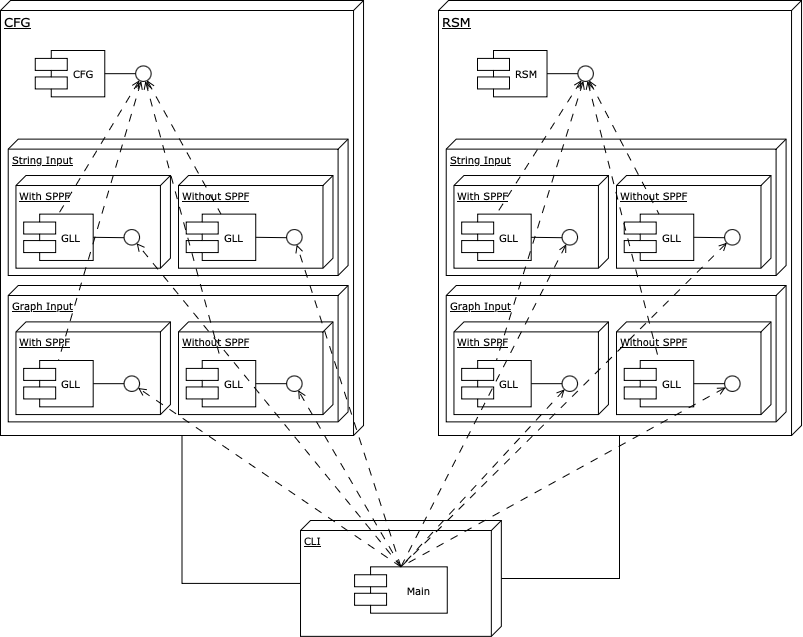
\includegraphics[width=\textwidth]{matmex-diploma-template-master/figures/architecture.png}
    \caption{Архитектура проекта}
    \label{fig:architecture}
\end{figure}

Разработанный проект имеет блочно-модульную архитектуру.
Диаграмма включает в себя три основных блока --- снизу блок, содеражащий модуль, реализующий интерфейс командой строки, который был отделен от модулей реализаций GLL, сверху слева блок, представляющий собой реализации GLL алгоритма на основе контекстно-свободных грамматик, имеющий общий модуль представления контекстно-свободной грамматики для всех GLL алгоритмов в блоке, сверху справа --- блок, представляющий собой реализации GLL алгоритма на основе рекурсивного автомата, имеющий общий модуль представления рекурсивного автомата для всех GLL алгоритмов в блоке.
Для обоих типов реализации были инкапсулированы в отдельные блоки сценарии выполнения алгоритма для входных данных в виде строки и для входных данных в виде графа.
Внутри последних в свою очередь были инкапсулированы сценарии с построением дерева разбора SPPF и без построения дерева разбора.

Данная архитектура позволяет не только максимально гибко задавать параметры для запуска алгоритма через интерфейс командой строки, но и облегчает понимание и поддержку кода, так как реализаци GLL алгоритмов имеют строгую иерархию и независимы между собой. 
\section{Экспериментальное исследование}\label{ps}

Для оценки производительности предложенного решения было проведено экспериментальное исследование на реальных графах и запросах.
В данном разделе приведены и описаны полученные результаты.

\subsection{Оборудование}
Все эксперименты были запущены на сервере со следующими характеристиками.

\begin{itemize}
    \item Операционная система Ubuntu 18.04.
    \item Процессор Intel Core i7-6700 CPU, 3.40GHz, 4 потока (hyper-thread-ing выключен).
    \item DDR4 64Gb RAM.
    \item OpenJDK 64-Bit виртуальная машина (build 25.362-b09, mixed mo-de). JVM сконфигурирована использовать 60Gb памяти кучи. 
\end{itemize}

\subsection{Эспериментальные данные}
Экспериментальное исследование проводилось на графах, содержащихся в библиотеке CFPQ\_Data\footnote{CFPQ\_Data --- это публичный набор графов и грамматик для CFPQ-алгоритмов. GitHub репозиторий: \url{https://github.com/FormalLanguageConstrainedPathQuerying/CFPQ_Data}. Accessed: 05/04/2023. }.
Был выбран набор графов, относящихся к RDF анализу (класс RDF), как достаточно известный и зарекомендовавший себя со временем набор графов для исследования решающих задачу поиска достижимостей в графе с контекстно-свободными ограничениями.
% , а также множество графов, извлеченных из исходного кода операционной системы Linux, относящихся к статическому анализу кода (класс MemoryAliases).
Подробное описание графов (количество вершин, ребер, а также количество ребер с метками, используемых в запросе) приведено в таблице~\ref{tab:graphs_for_evaluation_rdf}.


\begin{table*}
    \centering
    \resizebox{\columnwidth}{!}{%
    \begin{tabular}{| l | r | r | r | r | r | r |}
         \hline
         Название графа & $|V|$ & $|E|$ & \#subClassOf & \#type & \#broaderTransitive\\
         \hline
         \hline
            skos & 144 & 252 & 1 & 70 & 0 \\
            generations & 129 & 273 & 0 & 78 & 0 \\
            travel & 131 & 277 & 30 & 90 & 0 \\
            univ & 179 & 293 & 36 & 84 & 0 \\
            atom & 291 & 425 & 122 & 138 & 0 \\
            biomedical & 341 & 459 & 122 & 130 & 0 \\
            foaf & 256 & 631 & 10 & 174 & 0 \\
            people & 337 & 640 & 33 & 161 & 0 \\
            funding & 778 & 1086 & 90 & 304 & 0 \\
            wine & 733 & 1839 & 126 & 485 & 0 \\
            pizza & 671 & 1980 & 259 & 365 & 0 \\
            core & 1323 & 2752 & 178 & 706 & 0 \\
            pathways & 6238 & 12363 & 3117 & 3118 & 0 \\
            enzyme & 48815 & 86543 & 8163 & 14989 & 8156 \\
            eclass & 239111 & 360248 & 90962 & 72517 & 0 \\
            go\_hierarchy & 45007 & 490109 & 490109 & 0 & 0 \\
            go & 582929 & 1437437 & 94514 & 226481 & 0 \\
            geospecies & 450609 & 2201532 & 0 & 89062 & 20867 \\
            taxonomy & 5728398 & 14922125 & 2112637 & 2508635 & 0 \\
         \hline
    \end{tabular}%
    }
    \caption{Графы класса RDF: количество вершин, ребер и ребер с определенными метками}
    \label{tab:graphs_for_evaluation_rdf}
\end{table*}

%     \begin{table*}[h!]
%     \centering
%     \begin{tabular}{| c | c | c | c | c | c | c |}
%          \hline
%          Graph name & $|V|$ & $|E|$ & \#a & \#d \\
%          \hline
%          \hline
%          Apache         & 1 721 418 & 1 510 411  & 362 799 & 1 147 612 \\
%          Block          & 3 423 234 & 2 951 393  & 669 238 & 2 282 155 \\
%          Fs             & 4 177 416 & 3 609 373 & 824 430 & 2 784 943 \\
%          Ipc            & 3 401 022 & 2 931 498 & 664 151 & 2 267 347 \\
%          Lib            & 3 401 355 & 2 931 880 & 664 311 & 2 267 569 \\
%          Mm             & 2 538 243 & 2 191 079 & 498 918 & 1 692 161 \\
%          Net            & 4 039 470 & 3 500 141 & 807 162 & 2 692 979 \\
%          Postgre        & 5 203 419 & 4 678 543 & 1 209 597 & 3 468 946 \\
%          Security       & 3 479 982 & 3 003 326 & 683 339 & 2 319 987 \\
%          Sound          & 3 528 861 & 3 049 732 & 697 159 & 2 352 573 \\
%          Init           & 2 446 224 & 2 112 809 & 481 994 & 1 630 815 \\
%          Arch           & 3 448 422 & 2 970 242 & 6 712 95 & 2 298 947 \\
%          Crypto         & 3 464 970 & 2 988 387 & 678 408 & 2 309 979 \\
%          Drivers        & 4 273 803 & 3 707 769 & 858 568 & 2 849 201 \\
%          Kernel         & 11 254 434& 9 484 213  & 1 981 258 & 7 502 955 \\
%          \hline
%     \end{tabular}
%     \caption{Графы класса MemoryAliases: количество вершин, ребер и ребер с определенными метками}
%     \label{tab:graphs_for_evaluation_stat}
% \end{table*}


% Все использованные запросы являются вариациями запроса \emph{поиска потомков одного поколения}.
Для графов, из класса RDF были использованы те же запросы, что и в других работах по разработке алгоритмов решающих задачу поиска достижимостей в графе с контекстно-свободными ограничениями: $G_1$~(\ref{cfg:g_1}), $G_2$~(\ref{cfg:g_2}) и $Geo$~(\ref{cfg:geo}).
Запросы выражены как контекстно-свободные грамматики, где $S$ --- стартовый нетерминал, \textit{subClassOf, type, broaderTransitive, }$ \overline{\textit{subClassOf}}$, $\overline{\textit{type}}$, $\overline{\textit{broaderTransitive}}$ --- терминальные символы.
Здесь $\overline{x}$ обозначает обратное ребро $(v_j, x, v_i)$ для ребра $(v_i, x, v_j)$ в графе.
    
\begin{ruexample}
    Контекстно-свободная грамматика $G_1$.
    \begin{align}
    \begin{split}
    \label{cfg:g_1}
    S \to & \overline{\textit{subClassOf}} \ \ S \ \textit{subClassOf} \mid \overline{\textit{type}} \ \ S \ \textit{type}\\   & \mid \overline{\textit{subClassOf}} \ \ \textit{subClassOf} \mid \overline{\textit{type}} \ \textit{type}
    \end{split}
    \end{align}
\end{ruexample}

\begin{ruexample}
    Рекурсивный автомат $A_1$, соответствующий контекстно-свободной грамматике $G_1$.~
\end{ruexample}
\begin{align}
        \label{rsm:g_1}
        \begin{tikzpicture}[node distance=4cm,shorten >=1pt,on grid,auto]
           \node[state, initial] (q_0)   {$0 \{S\}$};
           \node[state] (q_1) [above right=of q_0] {$1 \{S\}$};
           \node[state] (q_2) [right=of q_1] {$2 \{S\}$};
           \node[state, accepting] (q_3) [below right=of q_2] {$3 \{S\}$};
           \node[state] (q_4) [below right=of q_0] {$4 \{S\}$};
           \node[state] (q_5) [right=of q_4] {$5 \{S\}$};
           \path[->]
            (q_0) edge[bend left, left]  node {$\overline{subClassOf}$} (q_1)
            (q_1) edge  node {$S$} (q_2)
            (q_2) edge[bend left, right]  node {$subClassOf$} (q_3)
            (q_1) edge[left]  node {$subClassOf$} (q_3)
            (q_0) edge[bend right, left] node {$\overline{type}$} (q_4)
            (q_4) edge  node {$S$} (q_5)
            (q_5) edge[bend right, right]  node {$type$} (q_3)
            (q_4) edge[left]  node {$type$} (q_3);
        \end{tikzpicture}
    \end{align}

\begin{ruexample}
    Контекстно-свободная грамматика $G_2$.
\begin{align}
\label{cfg:g_2}
S \to \overline{\textit{subClassOf}} \ \ S \ \textit{subClassOf} \mid \textit{subClassOf}
\end{align}
\end{ruexample}

\begin{ruexample}
    Рекурсивный автомат $A_2$, соответствующий контекстно-свободной грамматике $G_2$.~
    \begin{align}
    \label{rsm:g_2}
        \begin{tikzpicture}[node distance=4cm,shorten >=1pt,on grid,auto]
           \node[state, initial] (q_0)   {$0 \{S\}$};
           \node[state] (q_1) [right=of q_0] {$1 \{S\}$};
           \node[state] (q_2) [right=of q_1] {$2 \{S\}$};
           \node[state, accepting] (q_3) [right=of q_2] {$3 \{S\}$};
           \path[->]
            (q_0) edge[bend right, below]  node {$\overline{subClassOf}$} (q_1)
            (q_1) edge  node {$S$} (q_2)
            (q_2) edge[bend right, below]  node {$subClassOf$} (q_3)
            (q_0) edge[bend left, above]  node {$subClassOf$} (q_3);
        \end{tikzpicture}
    \end{align}
    
\end{ruexample}


\begin{ruexample}
    Контекстно-свободная грамматика $Geo$.
\begin{align}
\begin{split}
\label{cfg:geo}
S \to & \textit{broaderTransitive} \ \  S \ \overline{\textit{broaderTransitive}} \\
      & \mid \textit{broaderTransitive} \ \  \overline{\textit{broaderTransitive}}
\end{split}
\end{align}
\end{ruexample}

\begin{ruexample}
    Рекурсивный автомат $A_{geo}$, соответствующий контекстно-свободной грамматике $Geo$.~
\end{ruexample}

    \begin{align}
    \label{rsm:geo}
        \begin{tikzpicture}[node distance=4cm,shorten >=1pt,on grid,auto]
           \node[state, initial] (q_0)   {$0 \{S\}$};
           \node[state] (q_1) [right=of q_0] {$1 \{S\}$};
           \node[state] (q_2) [right=of q_1] {$2 \{S\}$};
           \node[state, accepting] (q_3) [right=of q_2] {$3 \{S\}$};
           \path[->]
            (q_0) edge[bend left, above]  node {$broaderTransitive$} (q_1)
            (q_1) edge  node {$S$} (q_2)
            (q_2) edge[bend right, below]  node {$\overline{broaderTransitive}$} (q_3)
            (q_1) edge[bend left, above]  node {$\overline{broaderTransitive}$} (q_3);
        \end{tikzpicture}
    \end{align}


% Для графов класса MemoryAliases был взят запрос $PointsTo ~(\ref{cfg:points_to})$, использовавшийся в исследовании~\cite{Zheng}. 
% \begin{ruexample}
%     Контекстно-свободная грамматика $PointsTo$.
% \begin{align}
% \begin{split}
% \label{cfg:points_to}
% S & \to \overline{d} \ V \ d \\
% V & \to V_1 \ V_2 \ V_3 \\
% V_1 & \to \varepsilon \\
% V_1 & \to V_2 \ \overline{a} \ V_1 \\
% V_2 & \to \varepsilon \\
% V_2 & \to S \\
% V_3 & \to \varepsilon \\
% V_3 & \to a \ V_2 \ V_3 \\
% \end{split}
% \end{align}
% \end{ruexample}

% \begin{ruexample}
%     Рекурсивный автомат $A_{PointsTo}$, соответствующий контекстно-свободной грамматике $PointsTo$.~
% \end{ruexample}

%     \begin{align}
%     \label{rsm:points_to}
%         \begin{tikzpicture}[node distance=2.7cm,shorten >=1pt,on grid,auto, x=20mm, y=20mm]
%            \node[state, initial] (q_0)   {$0 \{S\}$};
%            \node[state] (q_1) [right=of q_0] {$1 \{S\}$};
%            \node[state] (q_2) [right=of q_1] {$2 \{S\}$};
%            \node[state, accepting] (q_3) [right=of q_2] {$3 \{S\}$};
%            \node[state, initial, accepting] (q_4) [below=of q_0] {$4 \{V\}$};
%            \node[state] (q_5) [right=of q_4] {$5 \{V\}$};
%            \node[state, accepting] (q_6) [right=of q_5] {$6 \{V\}$};
%            \node[state, accepting] (q_7) [right=of q_6] {$7 \{V\}$};
%            \node[state, accepting] (q_8) [right=of q_7] {$8 \{V\}$};
%            \node[state, accepting] (q_9) [right=of q_8] {$9 \{V\}$};
%            \path[->]
%             (q_0) edge node {$\overline{d}$} (q_1)
%             (q_1) edge node {$V$} (q_2)
%             (q_2) edge node {$d$} (q_3)
%             (q_4) edge[out=270, in=270, looseness=1] node {$\overline{a}$} (q_6)
%             (q_4) edge[out=270, in=270, looseness=1] node {$a$} (q_8)
%             (q_4) edge node {$S$} (q_5)
%             (q_4) edge[out=270, in=270, looseness=1] node {$S$} (q_7)
%             (q_5) edge[bend right, below] node {$\overline{a}$} (q_6)
%             (q_6) edge[out=330, in=300, looseness=8] node {$\overline{a}$} (q_6)
%             (q_6) edge[bend left] node {$a$} (q_8)
%             (q_6) edge[bend right, above] node {$S$} (q_5)
%             (q_6) edge node {$S$} (q_7)
%             (q_7) edge node {$a$} (q_8)
%             (q_8) edge[out=330,in=300,looseness=8] node {$a$} (q_8)
%             (q_8) edge node {$S$} (q_9)
%             (q_9) edge[out=120, in=60, above] node {$a$} (q_8)
%             ;
%         \end{tikzpicture}
%     \end{align}

Кроме того, для исследования различий в эффективности обработки регулярных выражений классическим и модифицированным GLL алгоритмами, были выбраны следующие регулярные выражения, построенные по шаблонам $Q_1$, $Q_2$, $Q_{4}^{2}$ и $Q_6$ из работы~\cite{regex}. 

\begin{ruexample}
    Регулярное выражение $R_1$ для класса графов RDF, построенное по шаблону $Q_1$ на терминальном символе $type$.
\begin{align}
\begin{split}
\label{reg:rdf_reg_1}
type^*
\end{split}
\end{align}
\end{ruexample}

\begin{ruexample}
    Контекстно-свободная грамматика $G_{R_1}$, соответствующая регулярному выражению~(\ref{reg:rdf_reg_1}).
\begin{align}
\begin{split}
\label{cfg:rdf_reg_1}
S & \to \varepsilon \\
S & \to type \ S \\
\end{split}
\end{align}
\end{ruexample}

\begin{ruexample}
    Рекурсивный автомат $A_{R_1}$, соответствующий регулярному выражению~(\ref{reg:rdf_reg_1}).
\end{ruexample}

    \begin{align}
    \label{rsm:rdf_reg_1}
        \begin{tikzpicture}[node distance=2.7cm,shorten >=1pt,on grid,auto, x=20mm, y=20mm]
           \node[state, initial, accepting] (q_0)   {$0 \{S\}$};
           \path[->]
            (q_0) edge[out=30, in=150, looseness=8, above] node {$type$} (q_0)
            ;
        \end{tikzpicture}
    \end{align}

% \begin{ruexample}
%     Регулярное выражение для класса графов MemoryAliases, построенное по шаблону $Q_1$ на терминальном символе $a$.
% \begin{align}
% \begin{split}
% \label{reg:memory_aliases_reg_1}
% a^*
% \end{split}
% \end{align}
% \end{ruexample}

% \begin{ruexample}
%     Контекстно-свободная грамматика, соответствующая регулярному выражению~(\ref{reg:memory_aliases_reg_1}).
% \begin{align}
% \begin{split}
% \label{cfg:memory_aliases_reg_1}
% S & \to \varepsilon \\
% S & \to a \ S \\
% \end{split}
% \end{align}
% \end{ruexample}

% \begin{ruexample}
%     Рекурсивный автомат, соответствующий регулярному выражению~(\ref{reg:memory_aliases_reg_1}).
% \end{ruexample}

%     \begin{align}
%     \label{rsm:memory_aliases_reg_1}
%         \begin{tikzpicture}[node distance=2.7cm,shorten >=1pt,on grid,auto, x=20mm, y=20mm]
%            \node[state, initial, accepting] (q_0)   {$0 \{S\}$};
%            \path[->]
%             (q_0) edge[out=30, in=150, looseness=8, above] node {$a$} (q_0)
%             ;
%         \end{tikzpicture}
%     \end{align}

\begin{ruexample}
    Регулярное выражение $R_2$ для класса графов RDF, построенное по шаблону $Q_2$ на терминальных символах $type$ и $subClassOf$ соответственно.
\begin{align}
\begin{split}
\label{reg:rdf_reg_2}
type \ subClassOf^*
\end{split}
\end{align}
\end{ruexample}

\begin{ruexample}
    Контекстно-свободная грамматика $G_{R_2}$, соответствующая регулярному выражению~(\ref{reg:rdf_reg_2}).
\begin{align}
\begin{split}
\label{cfg:rdf_reg_2}
S & \to type \ C \\
C & \to \varepsilon \\
C & \to subClassOf \ C \\
\end{split}
\end{align}
\end{ruexample}

\begin{ruexample}
    Рекурсивный автомат $A_{R_2}$, соответствующий регулярному выражению~(\ref{reg:rdf_reg_2}).
\end{ruexample}

    \begin{align}
    \label{rsm:rdf_reg_2}
        \begin{tikzpicture}[node distance=4cm,shorten >=1pt,on grid,auto, x=20mm, y=20mm]
           \node[state, initial] (q_0)   {$0 \{S\}$};
           \node[state, accepting] (q_1) [right=of q_0]   {$1 \{S\}$};
           \path[->]
            (q_0) edge node {$type$} (q_1)
            (q_1) edge[out=30, in=150, looseness=8, above] node {$subClassOf$} (q_1)
            ;
        \end{tikzpicture}
    \end{align}

% \begin{ruexample}
%     Регулярное выражение для класса графов MemoryAliases, построенное по шаблону $Q_2$ на терминальных символах $a$ и $d$ соответственно.
% \begin{align}
% \begin{split}
% \label{reg:memory_aliases_reg_2}
% a \ d^*
% \end{split}
% \end{align}
% \end{ruexample}

% \begin{ruexample}
%     Контекстно-свободная грамматика, соответствующая регулярному выражению~(\ref{reg:memory_aliases_reg_2}).
% \begin{align}
% \begin{split}
% \label{cfg:memory_aliases_reg_2}
% S & \to a \ C \\
% C & \to \varepsilon \\
% C & \to d \ C \\
% \end{split}
% \end{align}
% \end{ruexample}

% \begin{ruexample}
%     Рекурсивный автомат, соответствующий регулярному выражению~(\ref{reg:memory_aliases_reg_2}).
% \end{ruexample}

%     \begin{align}
%     \label{rsm:memory_aliases_reg_2}
%         \begin{tikzpicture}[node distance=4cm,shorten >=1pt,on grid,auto, x=20mm, y=20mm]
%            \node[state, initial] (q_0)   {$0 \{S\}$};
%            \node[state, accepting] (q_1) [right=of q_0]   {$1 \{S\}$};
%            \path[->]
%             (q_0) edge node {$a$} (q_1)
%             (q_1) edge[out=30, in=150, looseness=8, above] node {$d$} (q_1)
%             ;
%         \end{tikzpicture}
%     \end{align}

\begin{ruexample}
    Регулярное выражение $R_3$ для класса графов RDF, построенное по шаблону $Q_{4}^{2}$ на терминальных символах $type$ и $subClassOf$ соответственно.
\begin{align}
\begin{split}
\label{reg:rdf_reg_3}
(type ~|~ subClassOf)^*
\end{split}
\end{align}
\end{ruexample}

\begin{ruexample}
    Контекстно-свободная грамматика $G_{R_3}$, соответствующая регулярному выражению~(\ref{reg:rdf_reg_3}).
\begin{align}
\begin{split}
\label{cfg:rdf_reg_3}
S & \to \varepsilon \\
S & \to type \ S \\
S & \to subClassOf \ S \\
\end{split}
\end{align}
\end{ruexample}

\begin{ruexample}
    Рекурсивный автомат $A_{R_3}$, соответствующий регулярному выражению~(\ref{reg:rdf_reg_3}).
\end{ruexample}

    \begin{align}
    \label{rsm:rdf_reg_3}
        \begin{tikzpicture}[node distance=2.7cm,shorten >=1pt,on grid,auto, x=20mm, y=20mm]
           \node[state, initial, accepting] (q_0)   {$0 \{S\}$};
           \path[->]
            (q_0) edge[out=30, in=150, looseness=8, above] node {$type$} (q_0)
            (q_0) edge[out=330, in=210, looseness=8, below] node {$subClassOf$} (q_0)
            ;
        \end{tikzpicture}
    \end{align}

% \begin{ruexample}
%     Регулярное выражение для класса графов MemoryAliases, построенное по шаблону $Q_{4}^{2}$ на терминальных символах $a$ и $d$ соответственно.
% \begin{align}
% \begin{split}
% \label{reg:memory_aliases_reg_3}
% (a ~|~ d)^*
% \end{split}
% \end{align}
% \end{ruexample}

% \begin{ruexample}
%     Контекстно-свободная грамматика, соответствующая регулярному выражению~(\ref{reg:memory_aliases_reg_3}).
% \begin{align}
% \begin{split}
% \label{cfg:memory_aliases_reg_3}
% S & \to \varepsilon \\
% S & \to a \ S \\
% S & \to d \ S \\
% \end{split}
% \end{align}
% \end{ruexample}

% \begin{ruexample}
%     Рекурсивный автомат, соответствующий регулярному выражению~(\ref{reg:memory_aliases_reg_3}).
% \end{ruexample}

%     \begin{align}
%     \label{rsm:memory_aliases_reg_3}
%         \begin{tikzpicture}[node distance=2.7cm,shorten >=1pt,on grid,auto, x=20mm, y=20mm]
%            \node[state, initial, accepting] (q_0)   {$0 \{S\}$};
%            \path[->]
%             (q_0) edge[out=30, in=150, looseness=8, above] node {$a$} (q_0)
%             (q_0) edge[out=330, in=210, looseness=8, below] node {$d$} (q_0)
%             ;
%         \end{tikzpicture}
%     \end{align}


\begin{ruexample}
    Регулярное выражение $R_4$ для класса графов RDF, построенное по шаблону $Q_6$на терминальных символах $type$ и $subClassOf$ соответственно.
\begin{align}
\begin{split}
\label{reg:rdf_reg_4}
type^* \ subClassOf^*
\end{split}
\end{align}
\end{ruexample}

\begin{ruexample}
    Контекстно-свободная грамматика $G_{R_4}$, соответствующая регулярному выражению~(\ref{reg:rdf_reg_4}).
\begin{align}
\begin{split}
\label{cfg:rdf_reg_4}
S & \to A \ B \\
A & \to \varepsilon \\
A & \to type \ A \\
B & \to \varepsilon \\
B & \to subClassOf \ B \\
\end{split}
\end{align}
\end{ruexample}

\begin{ruexample}
    Рекурсивный автомат $A_{R_4}$, соответствующий регулярному выражению~(\ref{reg:rdf_reg_4}).
\end{ruexample}

    \begin{align}
    \label{rsm:rdf_reg_4}
        \begin{tikzpicture}[node distance=5cm,shorten >=1pt,on grid,auto, x=20mm, y=20mm]
           \node[state, initial, accepting] (q_0)   {$0 \{S\}$};
           \node[state, accepting] (q_1) [right=of q_0]   {$1 \{S\}$};
           \path[->]
            (q_0) edge[out=30, in=150, looseness=4, above] node {$type$} (q_0)
            (q_0) edge node {$subClassOf$} (q_1)
            (q_1) edge[out=30, in=150, looseness=4, above] node {$subClassOf$} (q_1)
            ;
        \end{tikzpicture}
    \end{align}

% \begin{ruexample}
%     Регулярное выражение для класса графов MemoryAliases, построенное по шаблону $Q_6$ на терминальных символах $a$ и $d$ соответственно.
% \begin{align}
% \begin{split}
% \label{reg:memory_aliases_reg_4}
% a^* \ d^*
% \end{split}
% \end{align}
% \end{ruexample}

% \begin{ruexample}
%     Контекстно-свободная грамматика, соответствующая регулярному выражению~(\ref{reg:memory_aliases_reg_4}).
% \begin{align}
% \begin{split}
% \label{cfg:memory_aliases_reg_4}
% S & \to A \ B \\
% A & \to \varepsilon \\
% A & \to a \ A \\
% B & \to \varepsilon \\
% B & \to d \ B \\
% \end{split}
% \end{align}
% \end{ruexample}

% \begin{ruexample}
%     Рекурсивный автомат, соответствующий регулярному выражению~(\ref{reg:memory_aliases_reg_4}).
% \end{ruexample}

%     \begin{align}
%     \label{rsm:memory_aliases_reg_4}
%         \begin{tikzpicture}[node distance=5cm,shorten >=1pt,on grid,auto, x=20mm, y=20mm]
%            \node[state, initial] (q_0)   {$0 \{S\}$};
%            \node[state, accepting] (q_1) [right=of q_0]   {$1 \{S\}$};
%            \path[->]
%             (q_0) edge[out=30, in=150, looseness=4, above] node {$a$} (q_0)
%             (q_0) edge node {$d$} (q_1)
%             (q_1) edge[out=30, in=150, looseness=4, above] node {$d$} (q_1)
%             ;
%         \end{tikzpicture}
%     \end{align}

\subsection{Постановка экспериментов}

Экспериментальное исследование проводилось следующий образом.
\begin{itemize}
    \item Замерялось время работы классического и модифицированного GLL алгоритмов на задачах поиска путей в графе с контекст-но-свободными ограничениями, поиска достижимостей в графе с контекстно-свободными ограничениями и поиска достижимостей в графе с регулярными ограничениями.
    \item В качестве стартового и в качестве финального множеств запроса были расмотрены все вершины графа.
    \item В качестве контекстно-свободных ограничений были рассмотрены контекстно-свободные грамматики $G_1$~(\ref{cfg:g_1}), $G_2$~(\ref{cfg:g_2}), $Geo$~(\ref{cfg:geo}) и соответствующие им рекурсивные автоматы $A_1$~(\ref{rsm:g_1}), $A_2$~(\ref{rsm:g_2}), и $A_{geo}$~(\ref{rsm:geo}).
    \item В качестве регулярных ограничений были рассмотрены регулярные выражения $R_1$~(\ref{reg:rdf_reg_1}), $R_2$~(\ref{reg:rdf_reg_2}), $R_3$~(\ref{reg:rdf_reg_3}) и $R_4$~(\ref{reg:rdf_reg_4}), соответствующие им контекстно-свободные грамматики $G_{R_1}$~(\ref{cfg:rdf_reg_1}), $G_{R_2}$~(\ref{cfg:rdf_reg_2}), $G_{R_3}$~(\ref{cfg:rdf_reg_3}) и $G_{R_4}$~(\ref{cfg:rdf_reg_4}) представляли запросы для классического GLL алгоритма, а соответствующие им рекурсивные автоматы $A_{R_1}$~(\ref{rsm:rdf_reg_1}), $A_{R_2}$~(\ref{rsm:rdf_reg_2}), $A_{R_3}$~(\ref{rsm:rdf_reg_3}) и $A_{R_4}$~(\ref{rsm:rdf_reg_4}) представляли запросы для модифицированного GLL алгоритма.
    \item Для каждой четверки (граф, грамматика, GLL алгоритм, задача) проводилось 20 замеров времени работы в наносекундах.
\end{itemize}

\subsection{Результаты экспериментов}

Для удобства исследования полученные результаты были оформлены в виде таблиц, представленных ниже.
Результаты приведены с точностью до последней значащей цифры, выбранной с учетом стандартного отклонения для каждой выборки результатов.

Ниже представлены результаты работы классического GLL алгоритма в сравнении с модифицированным алгоритмом для сценария поиска всех путей и сценария поиска всех достижимостей на графах класса RDF с контекстно-свободными ограничениями.


% Please add the following required packages to your document preamble:
% \usepackage{multirow}
\begin{landscape}
\begin{table}[]
\resizebox{\columnwidth}{!}{%
\begin{tabular}{|l|rrrrrr|}
\hline
\multicolumn{1}{|c|}{\multirow{3}{*}{\begin{tabular}[c]{@{}c@{}}Название\\ графа\end{tabular}}} &
  \multicolumn{6}{c|}{Время в секундах} \\ \cline{2-7} 
\multicolumn{1}{|c|}{} &
  \multicolumn{2}{c|}{G1} &
  \multicolumn{2}{c|}{G2} &
  \multicolumn{2}{c|}{Geo} \\ \cline{2-7} 
\multicolumn{1}{|c|}{} &
  \multicolumn{1}{c|}{CFG} &
  \multicolumn{1}{c|}{RSM} &
  \multicolumn{1}{c|}{CFG} &
  \multicolumn{1}{c|}{RSM} &
  \multicolumn{1}{c|}{CFG} &
  \multicolumn{1}{c|}{RSM} \\ \hline
skos &
  \multicolumn{1}{r|}{$0.00021 \pm 0.00004$} &
  \multicolumn{1}{r|}{$0.0001 \pm 0.000005$} &
  \multicolumn{1}{r|}{$0.000038 \pm 0.000006$} &
  \multicolumn{1}{r|}{$0.000023 \pm 0.000004$} &
  \multicolumn{1}{r|}{$0.000037 \pm 0.000009$} &
  $0.000021 \pm 0.000005$ \\ \hline
generations &
  \multicolumn{1}{r|}{$0.000713 \pm 0.001008$} &
  \multicolumn{1}{r|}{$0.000226 \pm 0.000005$} &
  \multicolumn{1}{r|}{$0.000105 \pm 0.000018$} &
  \multicolumn{1}{r|}{$0.000086 \pm 0.000008$} &
  \multicolumn{1}{r|}{$0.00009 \pm 0.000008$} &
  $0.000064 \pm 0.000006$ \\ \hline
travel &
  \multicolumn{1}{r|}{$0.00079 \pm 0.00004$} &
  \multicolumn{1}{r|}{$0.000425 \pm 0.000007$} &
  \multicolumn{1}{r|}{$0.00028 \pm 0.00002$} &
  \multicolumn{1}{r|}{$0.000255 \pm 0.000006$} &
  \multicolumn{1}{r|}{$0.000092 \pm 0.000006$} &
  $0.000066 \pm 0.000011$ \\ \hline
univ &
  \multicolumn{1}{r|}{$0.0009 \pm 0.0003$} &
  \multicolumn{1}{r|}{$0.000416 \pm 0.000010$} &
  \multicolumn{1}{r|}{$0.00036 \pm 0.00003$} &
  \multicolumn{1}{r|}{$0.000273 \pm 0.000019$} &
  \multicolumn{1}{r|}{$0.00013 \pm 0.00002$} &
  $0.00009 \pm 0.000010$ \\ \hline
atom &
  \multicolumn{1}{r|}{$0.00058 \pm 0.00007$} &
  \multicolumn{1}{r|}{$0.000261 \pm 0.000012$} &
  \multicolumn{1}{r|}{$0.00028 \pm 0.00002$} &
  \multicolumn{1}{r|}{$0.000211 \pm 0.000010$} &
  \multicolumn{1}{r|}{$0.000078 \pm 0.000019$} &
  $0.000047 \pm 0.000012$ \\ \hline
biomedical &
  \multicolumn{1}{r|}{$0.00181 \pm 0.00018$} &
  \multicolumn{1}{r|}{$0.001 \pm 0.0002$} &
  \multicolumn{1}{r|}{$0.0012 \pm 0.0004$} &
  \multicolumn{1}{r|}{$0.00082 \pm 0.00006$} &
  \multicolumn{1}{r|}{$0.000232 \pm 0.000012$} &
  $0.000161 \pm 0.000014$ \\ \hline
foaf &
  \multicolumn{1}{r|}{$0.0015 \pm 0.0006$} &
  \multicolumn{1}{r|}{$0.00074 \pm 0.00004$} &
  \multicolumn{1}{r|}{$0.00029 \pm 0.00003$} &
  \multicolumn{1}{r|}{$0.0002 \pm 0.00002$} &
  \multicolumn{1}{r|}{$0.00021 \pm 0.00004$} &
  $0.00013 \pm 0.00002$ \\ \hline
people &
  \multicolumn{1}{r|}{$0.00133 \pm 0.00003$} &
  \multicolumn{1}{r|}{$0.0007 \pm 0.00003$} &
  \multicolumn{1}{r|}{$0.00047 \pm 0.00005$} &
  \multicolumn{1}{r|}{$0.0004 \pm 0.00002$} &
  \multicolumn{1}{r|}{$0.00023 \pm 0.00002$} &
  $0.00016 \pm 0.00002$ \\ \hline
funding &
  \multicolumn{1}{r|}{$0.00118 \pm 0.00009$} &
  \multicolumn{1}{r|}{$0.0005 \pm 0.0002$} &
  \multicolumn{1}{r|}{$0.0004 \pm 0.00005$} &
  \multicolumn{1}{r|}{$0.00026 \pm 0.00002$} &
  \multicolumn{1}{r|}{$0.0004 \pm 0.0003$} &
  $0.00013 \pm 0.00003$ \\ \hline
wine &
  \multicolumn{1}{r|}{$0.0028 \pm 0.0007$} &
  \multicolumn{1}{r|}{$0.0031 \pm 0.0002$} &
  \multicolumn{1}{r|}{$0.0019 \pm 0.0003$} &
  \multicolumn{1}{r|}{$0.00156 \pm 0.00016$} &
  \multicolumn{1}{r|}{$0.00053 \pm 0.00002$} &
  $0.00037 \pm 0.00004$ \\ \hline
pizza &
  \multicolumn{1}{r|}{$0.0065 \pm 0.0005$} &
  \multicolumn{1}{r|}{$0.0053 \pm 0.0004$} &
  \multicolumn{1}{r|}{$0.004 \pm 0.0006$} &
  \multicolumn{1}{r|}{$0.0031 \pm 0.00018$} &
  \multicolumn{1}{r|}{$0.0005 \pm 0.00014$} &
  $0.00033 \pm 0.00002$ \\ \hline
core &
  \multicolumn{1}{r|}{$0.0094 \pm 0.0009$} &
  \multicolumn{1}{r|}{$0.0055 \pm 0.0011$} &
  \multicolumn{1}{r|}{$0.0034 \pm 0.0006$} &
  \multicolumn{1}{r|}{$0.0028 \pm 0.0004$} &
  \multicolumn{1}{r|}{$0.0015 \pm 0.0006$} &
  $0.0012 \pm 0.0003$ \\ \hline
pathways &
  \multicolumn{1}{r|}{$0.04 \pm 0.004$} &
  \multicolumn{1}{r|}{$0.02 \pm 0.004$} &
  \multicolumn{1}{r|}{$0.03 \pm 0.009$} &
  \multicolumn{1}{r|}{$0.01104 \pm 0.00103$} &
  \multicolumn{1}{r|}{$0.00255 \pm 0.00013$} &
  $0.00153 \pm 0.00016$ \\ \hline
enzyme &
  \multicolumn{1}{r|}{$0.16 \pm 0.03$} &
  \multicolumn{1}{r|}{$0.076 \pm 0.019$} &
  \multicolumn{1}{r|}{$0.062 \pm 0.008$} &
  \multicolumn{1}{r|}{$0.049 \pm 0.009$} &
  \multicolumn{1}{r|}{$54.7 \pm 1.4$} &
  $53.7 \pm 1.2$ \\ \hline
eclass &
  \multicolumn{1}{r|}{$1.8 \pm 0.3$} &
  \multicolumn{1}{r|}{$0.91 \pm 0.18$} &
  \multicolumn{1}{r|}{$0.9 \pm 0.17$} &
  \multicolumn{1}{r|}{$0.68 \pm 0.12$} &
  \multicolumn{1}{r|}{$0.23 \pm 0.18$} &
  $0.13 \pm 0.03$ \\ \hline
go\_hierarchy &
  \multicolumn{1}{r|}{$23.83 \pm 1.03$} &
  \multicolumn{1}{r|}{$19.9 \pm 0.7$} &
  \multicolumn{1}{r|}{$21.6 \pm 0.8$} &
  \multicolumn{1}{r|}{$19.4 \pm 0.7$} &
  \multicolumn{1}{r|}{$0.0296 \pm 0.0014$} &
  $0.016 \pm 0.004$ \\ \hline
go &
  \multicolumn{1}{r|}{OOM} &
  \multicolumn{1}{r|}{OOM} &
  \multicolumn{1}{r|}{OOM} &
  \multicolumn{1}{r|}{OOM} &
  \multicolumn{1}{r|}{$0.48 \pm 0.06$} &
  $0.27 \pm 0.07$ \\ \hline
geospecies &
  \multicolumn{1}{r|}{OOM} &
  \multicolumn{1}{r|}{OOM} &
  \multicolumn{1}{r|}{OOM} &
  \multicolumn{1}{r|}{OOM} &
  \multicolumn{1}{r|}{OOM} &
  OOM \\ \hline
taxonomy &
  \multicolumn{1}{r|}{OOM} &
  \multicolumn{1}{r|}{OOM} &
  \multicolumn{1}{r|}{OOM} &
  \multicolumn{1}{r|}{OOM} &
  \multicolumn{1}{r|}{$7.7 \pm 0.4$} &
  $4.4 \pm 0.5$ \\ \hline
\end{tabular}%
}
\caption{Результаты экспериментов на задаче поиска путей в графе с контекстно-свободными ограничениями}
\label{tab:results_with_sppf}
\end{table}
\end{landscape}

% Please add the following required packages to your document preamble:
% \usepackage{multirow}
\begin{landscape}
\begin{table}[]
\resizebox{\columnwidth}{!}{%
\begin{tabular}{|l|rrrrrr|}
\hline
\multicolumn{1}{|c|}{\multirow{3}{*}{\begin{tabular}[c]{@{}c@{}}Название\\ графа\end{tabular}}} &
  \multicolumn{6}{c|}{Время в секундах} \\ \cline{2-7} 
\multicolumn{1}{|c|}{} &
  \multicolumn{2}{c|}{G1} &
  \multicolumn{2}{c|}{G2} &
  \multicolumn{2}{c|}{Geo} \\ \cline{2-7} 
\multicolumn{1}{|c|}{} &
  \multicolumn{1}{c|}{CFG} &
  \multicolumn{1}{c|}{RSM} &
  \multicolumn{1}{c|}{CFG} &
  \multicolumn{1}{c|}{RSM} &
  \multicolumn{1}{c|}{CFG} &
  \multicolumn{1}{c|}{RSM} \\ \hline
skos &
  \multicolumn{1}{r|}{$0.00027 \pm 0.00002$} &
  \multicolumn{1}{r|}{$0.00005 \pm 0.000002$} &
  \multicolumn{1}{r|}{$0.000039 \pm 0.000010$} &
  \multicolumn{1}{r|}{$0.000027 \pm 0.000011$} &
  \multicolumn{1}{r|}{$0.000055 \pm 0.000005$} &
  $0.000024 \pm 0.000010$ \\ \hline
generations &
  \multicolumn{1}{r|}{$0.00047 \pm 0.00004$} &
  \multicolumn{1}{r|}{$0.00017 \pm 0.000010$} &
  \multicolumn{1}{r|}{$0.00013 \pm 0.00002$} &
  \multicolumn{1}{r|}{$0.000077 \pm 0.000014$} &
  \multicolumn{1}{r|}{$0.000082 \pm 0.000001$} &
  $0.000069 \pm 0.000019$ \\ \hline
travel &
  \multicolumn{1}{r|}{$0.00051 \pm 0.00004$} &
  \multicolumn{1}{r|}{$0.000267 \pm 0.000014$} &
  \multicolumn{1}{r|}{$0.00025 \pm 0.00002$} &
  \multicolumn{1}{r|}{$0.000149 \pm 0.000018$} &
  \multicolumn{1}{r|}{$0.000091 \pm 0.000013$} &
  $0.000069 \pm 0.000010$ \\ \hline
univ &
  \multicolumn{1}{r|}{$0.00062 \pm 0.000021$} &
  \multicolumn{1}{r|}{$0.0003 \pm 0.00005$} &
  \multicolumn{1}{r|}{$0.00026 \pm 0.00004$} &
  \multicolumn{1}{r|}{$0.00019 \pm 0.00002$} &
  \multicolumn{1}{r|}{$0.000133 \pm 0.000015$} &
  $0.000086 \pm 0.000010$ \\ \hline
atom &
  \multicolumn{1}{r|}{$0.000711 \pm 0.000053$} &
  \multicolumn{1}{r|}{$0.000133 \pm 0.000002$} &
  \multicolumn{1}{r|}{$0.000168 \pm 0.000011$} &
  \multicolumn{1}{r|}{$0.000116 \pm 0.000018$} &
  \multicolumn{1}{r|}{$0.000124 \pm 0.000018$} &
  $0.000038 \pm 0.000005$ \\ \hline
biomedical &
  \multicolumn{1}{r|}{$0.00124 \pm 0.00007$} &
  \multicolumn{1}{r|}{$0.00059 \pm 0.00007$} &
  \multicolumn{1}{r|}{$0.00081 \pm 0.00008$} &
  \multicolumn{1}{r|}{$0.00056 \pm 0.00007$} &
  \multicolumn{1}{r|}{$0.000238 \pm 0.000017$} &
  $0.000161 \pm 0.000014$ \\ \hline
foaf &
  \multicolumn{1}{r|}{$0.00082 \pm 0.00004$} &
  \multicolumn{1}{r|}{$0.00041 \pm 0.00004$} &
  \multicolumn{1}{r|}{$0.00026 \pm 0.00003$} &
  \multicolumn{1}{r|}{$0.000190 \pm 0.000015$} &
  \multicolumn{1}{r|}{$0.0002 \pm 0.00004$} &
  $0.000144 \pm 0.000014$ \\ \hline
people &
  \multicolumn{1}{r|}{$0.001 \pm 0.0002$} &
  \multicolumn{1}{r|}{$0.00051 \pm 0.00008$} &
  \multicolumn{1}{r|}{$0.00046 \pm 0.00004$} &
  \multicolumn{1}{r|}{$0.000261 \pm 0.000013$} &
  \multicolumn{1}{r|}{$0.00023 \pm 0.00002$} &
  $0.00015 \pm 0.00002$ \\ \hline
funding &
  \multicolumn{1}{r|}{$0.001551 \pm 0.000109$} &
  \multicolumn{1}{r|}{$0.000294 \pm 0.000006$} &
  \multicolumn{1}{r|}{$0.00028 \pm 0.00002$} &
  \multicolumn{1}{r|}{$0.000187 \pm 0.000016$} &
  \multicolumn{1}{r|}{$0.000244 \pm 0.000019$} &
  $0.00013 \pm 0.00002$ \\ \hline
wine &
  \multicolumn{1}{r|}{$0.0035 \pm 0.0003$} &
  \multicolumn{1}{r|}{$0.001639 \pm 0.000103$} &
  \multicolumn{1}{r|}{$0.0015 \pm 0.00011$} &
  \multicolumn{1}{r|}{$0.00081 \pm 0.00007$} &
  \multicolumn{1}{r|}{$0.00048 \pm 0.00003$} &
  $0.00035 \pm 0.00003$ \\ \hline
pizza &
  \multicolumn{1}{r|}{$0.0045 \pm 0.0009$} &
  \multicolumn{1}{r|}{$0.00051 \pm 0.00008$} &
  \multicolumn{1}{r|}{$0.00211 \pm 0.00015$} &
  \multicolumn{1}{r|}{$0.0015 \pm 0.0002$} &
  \multicolumn{1}{r|}{$0.00046 \pm 0.00002$} &
  $0.00031 \pm 0.00002$ \\ \hline
core &
  \multicolumn{1}{r|}{$0.0054 \pm 0.0007$} &
  \multicolumn{1}{r|}{$0.0031 \pm 0.0009$} &
  \multicolumn{1}{r|}{$0.0027 \pm 0.0004$} &
  \multicolumn{1}{r|}{$0.002 \pm 0.0004$} &
  \multicolumn{1}{r|}{$0.0014 \pm 0.0004$} &
  $0.0012 \pm 0.0004$ \\ \hline
pathways &
  \multicolumn{1}{r|}{$0.0169 \pm 0.0016$} &
  \multicolumn{1}{r|}{$0.0077 \pm 0.0003$} &
  \multicolumn{1}{r|}{$0.0088 \pm 0.0007$} &
  \multicolumn{1}{r|}{$0.00606 \pm 0.00019$} &
  \multicolumn{1}{r|}{$0.0026 \pm 0.0002$} &
  $0.0018 \pm 0.0002$ \\ \hline
enzyme &
  \multicolumn{1}{r|}{$0.107 \pm 0.007$} &
  \multicolumn{1}{r|}{$0.044 \pm 0.008$} &
  \multicolumn{1}{r|}{$0.049 \pm 0.006$} &
  \multicolumn{1}{r|}{$0.039 \pm 0.014$} &
  \multicolumn{1}{r|}{$8.6 \pm 0.8$} &
  $8.36 \pm 1.02$ \\ \hline
eclass &
  \multicolumn{1}{r|}{$0.943649 \pm 0.14$} &
  \multicolumn{1}{r|}{$0.43 \pm 0.07$} &
  \multicolumn{1}{r|}{$0.51 \pm 0.11$} &
  \multicolumn{1}{r|}{$0.39 \pm 0.07$} &
  \multicolumn{1}{r|}{$0.21 \pm 0.18$} &
  $0.13 \pm 0.12$ \\ \hline
go\_hierarchy &
  \multicolumn{1}{r|}{$4.1 \pm 0.6$} &
  \multicolumn{1}{r|}{$3.0 \pm 0.4$} &
  \multicolumn{1}{r|}{$3.71 \pm 0.15$} &
  \multicolumn{1}{r|}{$3.5 \pm 0.2$} &
  \multicolumn{1}{r|}{$0.0272 \pm 0.0015$} &
  $0.0301 \pm 0.0011$ \\ \hline
go &
  \multicolumn{1}{r|}{$3.2 \pm 0.3$} &
  \multicolumn{1}{r|}{$1.86 \pm 0.16$} &
  \multicolumn{1}{r|}{$1.8 \pm 0.3$} &
  \multicolumn{1}{r|}{$1.49 \pm 0.13$} &
  \multicolumn{1}{r|}{$0.45 \pm 0.07$} &
  $0.28 \pm 0.18$ \\ \hline
geospecies &
  \multicolumn{1}{r|}{$0.97 \pm 0.12$} &
  \multicolumn{1}{r|}{$0.34 \pm 0.04$} &
  \multicolumn{1}{r|}{$0.36 \pm 0.08$} &
  \multicolumn{1}{r|}{$0.25 \pm 0.05$} &
  \multicolumn{1}{r|}{$279.2 \pm 11.4$} &
  $275.5 \pm 4.6$ \\ \hline
taxonomy &
  \multicolumn{1}{r|}{$31.2 \pm 1.5$} &
  \multicolumn{1}{r|}{$14.8 \pm 0.6$} &
  \multicolumn{1}{r|}{$17.7 \pm 0.8$} &
  \multicolumn{1}{r|}{$13.7 \pm 0.6$} &
  \multicolumn{1}{r|}{$6.9 \pm 0.6$} &
  $4.1 \pm 0.6$ \\ \hline
\end{tabular}%
}
\caption{Результаты экспериментов на задаче поиска достижимостей в графе с контекстно-свободными ограничениями}
\label{tab:results_without_sppf}
\end{table}
\end{landscape}

Здесь $OOM$ означает $Out \ of \ Memory$, то есть то, что для обработки графа оказалось недостаточно оперативной памяти.

Из полученных результатов можно сделать следующие выводы.
\begin{itemize}
    \item Прежде всего, стоит заметить, что предоставленные модификации эффективны в контексте применимости алгоритма. В подавляющем большинстве случаев использование рекурсивного автомата дало положительный результат на времени работы GLL алгоритма. 
    \item Как для классического GLL, так и для модифицированного большое значение имеет сруктура графа. Так, чем большее количество вершин содержит граф, тем сильнее на нем отражается улучшение во времени работы. Однако для относительно плотных графов (например, $go\_hierarchy$) ускорение заметно не так сильно.
    \item Значимым результатом является то, что модифицированный алгоритм работает быстрее не только на графах с большим количеством вершин, но также и на графах с запросами, возвращающими большое количество пар достижимостей ($go,~taxonomy$). Так, например, на графе $taxonomy$ и запросе $G_1$ можно наблюдать прирост в производительности более, чем в два раза.
\end{itemize}

Ниже представлены результаты работы классического GLL алгоритма в сравнении с модифицированным алгоритмом для поиска всех достижимостей на графах класса RDF с регулярными ограничениями.

% Please add the following required packages to your document preamble:
% \usepackage{multirow}

% Please add the following required packages to your document preamble:
% \usepackage{multirow}
\begin{landscape}
\begin{table}[]
\resizebox{\columnwidth}{!}{%
\begin{tabular}{|l|rrrrrrrr|}
\hline
\multicolumn{1}{|c|}{\multirow{3}{*}{\begin{tabular}[c]{@{}c@{}}Название\\ графа\end{tabular}}} &
  \multicolumn{8}{c|}{Время в секундах} \\ \cline{2-9} 
\multicolumn{1}{|c|}{} &
  \multicolumn{2}{c|}{R1} &
  \multicolumn{2}{c|}{R2} &
  \multicolumn{2}{c|}{R3} &
  \multicolumn{2}{c|}{R4} \\ \cline{2-9} 
\multicolumn{1}{|c|}{} &
  \multicolumn{1}{c|}{CFG} &
  \multicolumn{1}{c|}{RSM} &
  \multicolumn{1}{c|}{CFG} &
  \multicolumn{1}{c|}{RSM} &
  \multicolumn{1}{c|}{CFG} &
  \multicolumn{1}{c|}{RSM} &
  \multicolumn{1}{c|}{CFG} &
  \multicolumn{1}{c|}{RSM} \\ \hline
skos &
  \multicolumn{1}{r|}{$0.000096 \pm 0.000019$} &
  \multicolumn{1}{r|}{$0.000160 \pm 0.000019$} &
  \multicolumn{1}{r|}{$0.00009 \pm 0.00002$} &
  \multicolumn{1}{r|}{$0.000041 \pm 0.000014$} &
  \multicolumn{1}{r|}{$0.000117 \pm 0.000018$} &
  \multicolumn{1}{r|}{$0.000062 \pm 0.000012$} &
  \multicolumn{1}{r|}{$0.0003 \pm 0.00003$} &
  $0.000056 \pm 0.000013$ \\ \hline
generations &
  \multicolumn{1}{r|}{$0.00027 \pm 0.00013$} &
  \multicolumn{1}{r|}{$0.000143 \pm 0.000016$} &
  \multicolumn{1}{r|}{$0.0004 \pm 0.0005$} &
  \multicolumn{1}{r|}{$0.000112 \pm 0.000014$} &
  \multicolumn{1}{r|}{$0.000276 \pm 0.000005$} &
  \multicolumn{1}{r|}{$0.000142 \pm 0.000004$} &
  \multicolumn{1}{r|}{$0.0003 \pm 0.00004$} &
  $0.000145 \pm 0.000003$ \\ \hline
travel &
  \multicolumn{1}{r|}{$0.00025 \pm 0.00002$} &
  \multicolumn{1}{r|}{$0.00015 \pm 0.00002$} &
  \multicolumn{1}{r|}{$0.00038 \pm 0.00002$} &
  \multicolumn{1}{r|}{$0.000133 \pm 0.000016$} &
  \multicolumn{1}{r|}{$0.000376 \pm 0.000018$} &
  \multicolumn{1}{r|}{$0.000180 \pm 0.000013$} &
  \multicolumn{1}{r|}{$0.00067 \pm 0.00017$} &
  $0.000176 \pm 0.000013$ \\ \hline
univ &
  \multicolumn{1}{r|}{$0.000331 \pm 0.000018$} &
  \multicolumn{1}{r|}{$0.0002 \pm 0.0002$} &
  \multicolumn{1}{r|}{$0.00039 \pm 0.00006$} &
  \multicolumn{1}{r|}{$0.000171 \pm 0.000010$} &
  \multicolumn{1}{r|}{$0.00047 \pm 0.00002$} &
  \multicolumn{1}{r|}{$0.00027 \pm 0.00002$} &
  \multicolumn{1}{r|}{$0.00094 \pm 0.00007$} &
  $0.00025 \pm 0.00003$ \\ \hline
atom &
  \multicolumn{1}{r|}{$0.00016 \pm 0.00002$} &
  \multicolumn{1}{r|}{$0.00028 \pm 0.00002$} &
  \multicolumn{1}{r|}{$0.000168 \pm 0.000015$} &
  \multicolumn{1}{r|}{$0.000076 \pm 0.000010$} &
  \multicolumn{1}{r|}{$0.00033 \pm 0.00005$} &
  \multicolumn{1}{r|}{$0.000120 \pm 0.000016$} &
  \multicolumn{1}{r|}{$0.00063 \pm 0.00005$} &
  $0.000132 \pm 0.000017$ \\ \hline
biomedical &
  \multicolumn{1}{r|}{$0.00065 \pm 0.00006$} &
  \multicolumn{1}{r|}{$0.00041 \pm 0.00017$} &
  \multicolumn{1}{r|}{$0.00067 \pm 0.00005$} &
  \multicolumn{1}{r|}{$0.00032 \pm 0.00002$} &
  \multicolumn{1}{r|}{$0.00117 \pm 0.00008$} &
  \multicolumn{1}{r|}{$0.00056 \pm 0.00004$} &
  \multicolumn{1}{r|}{$0.00205 \pm 0.00015$} &
  $0.00051 \pm 0.00002$ \\ \hline
foaf &
  \multicolumn{1}{r|}{$0.00058 \pm 0.00005$} &
  \multicolumn{1}{r|}{$0.000355 \pm 0.000017$} &
  \multicolumn{1}{r|}{$0.000667 \pm 0.000105$} &
  \multicolumn{1}{r|}{$0.00031 \pm 0.00005$} &
  \multicolumn{1}{r|}{$0.000734 \pm 0.000100$} &
  \multicolumn{1}{r|}{$0.00041 \pm 0.00014$} &
  \multicolumn{1}{r|}{$0.00136 \pm 0.00004$} &
  $0.00036 \pm 0.00002$ \\ \hline
people &
  \multicolumn{1}{r|}{$0.00061 \pm 0.00002$} &
  \multicolumn{1}{r|}{$0.000368 \pm 0.000019$} &
  \multicolumn{1}{r|}{$0.00084 \pm 0.00016$} &
  \multicolumn{1}{r|}{$0.0003 \pm 0.00004$} &
  \multicolumn{1}{r|}{$0.000799 \pm 0.000019$} &
  \multicolumn{1}{r|}{$0.00042 \pm 0.00003$} &
  \multicolumn{1}{r|}{$0.0016 \pm 0.0008$} &
  $0.00042 \pm 0.00004$ \\ \hline
funding &
  \multicolumn{1}{r|}{$0.00045 \pm 0.00004$} &
  \multicolumn{1}{r|}{$0.00083 \pm 0.00009$} &
  \multicolumn{1}{r|}{$0.00044 \pm 0.00005$} &
  \multicolumn{1}{r|}{$0.000210 \pm 0.000019$} &
  \multicolumn{1}{r|}{$0.0007 \pm 0.00007$} &
  \multicolumn{1}{r|}{$0.00036 \pm 0.00004$} &
  \multicolumn{1}{r|}{$0.001745 \pm 0.000106$} &
  $0.00035 \pm 0.00005$ \\ \hline
wine &
  \multicolumn{1}{r|}{$0.0018 \pm 0.0007$} &
  \multicolumn{1}{r|}{$0.00094 \pm 0.00009$} &
  \multicolumn{1}{r|}{$0.0025 \pm 0.0002$} &
  \multicolumn{1}{r|}{$0.000845 \pm 0.000109$} &
  \multicolumn{1}{r|}{$0.0023 \pm 0.0002$} &
  \multicolumn{1}{r|}{$0.0012 \pm 0.00007$} &
  \multicolumn{1}{r|}{$0.0029 \pm 0.0004$} &
  $0.0012 \pm 0.0003$ \\ \hline
pizza &
  \multicolumn{1}{r|}{$0.002 \pm 0.0002$} &
  \multicolumn{1}{r|}{$0.001 \pm 0.0002$} &
  \multicolumn{1}{r|}{$0.002 \pm 0.0001$} &
  \multicolumn{1}{r|}{$0.00079 \pm 0.00006$} &
  \multicolumn{1}{r|}{$0.0023 \pm 0.0002$} &
  \multicolumn{1}{r|}{$0.00111 \pm 0.00003$} &
  \multicolumn{1}{r|}{$0.0044 \pm 0.0002$} &
  $0.00109 \pm 0.00005$ \\ \hline
core &
  \multicolumn{1}{r|}{$0.005 \pm 0.0003$} &
  \multicolumn{1}{r|}{$0.003 \pm 0.0004$} &
  \multicolumn{1}{r|}{$0.0042 \pm 0.0005$} &
  \multicolumn{1}{r|}{$0.0019 \pm 0.0002$} &
  \multicolumn{1}{r|}{$0.0054 \pm 0.0006$} &
  \multicolumn{1}{r|}{$0.0031 \pm 0.0005$} &
  \multicolumn{1}{r|}{$0.012 \pm 0.004$} &
  $0.0031 \pm 0.0003$ \\ \hline
pathways &
  \multicolumn{1}{r|}{$0.0063 \pm 0.0003$} &
  \multicolumn{1}{r|}{$0.0068 \pm 0.0107$} &
  \multicolumn{1}{r|}{$0.0141 \pm 0.0011$} &
  \multicolumn{1}{r|}{$0.00631 \pm 0.00015$} &
  \multicolumn{1}{r|}{$0.0162 \pm 0.0014$} &
  \multicolumn{1}{r|}{$0.0078 \pm 0.0004$} &
  \multicolumn{1}{r|}{$0.06 \pm 0.009$} &
  $0.0082 \pm 0.0005$ \\ \hline
enzyme &
  \multicolumn{1}{r|}{$0.06 \pm 0.011$} &
  \multicolumn{1}{r|}{$0.0407 \pm 0.0108$} &
  \multicolumn{1}{r|}{$0.061 \pm 0.011$} &
  \multicolumn{1}{r|}{$0.032 \pm 0.011$} &
  \multicolumn{1}{r|}{$0.11 \pm 0.02$} &
  \multicolumn{1}{r|}{$0.056 \pm 0.007$} &
  \multicolumn{1}{r|}{$0.31 \pm 0.08$} &
  $0.0577 \pm 0.0102$ \\ \hline
eclass &
  \multicolumn{1}{r|}{$0.43 \pm 0.11$} &
  \multicolumn{1}{r|}{$0.28 \pm 0.08$} &
  \multicolumn{1}{r|}{$0.44 \pm 0.11$} &
  \multicolumn{1}{r|}{$0.19 \pm 0.05$} &
  \multicolumn{1}{r|}{$0.94 \pm 0.17$} &
  \multicolumn{1}{r|}{$0.50 \pm 0.09$} &
  \multicolumn{1}{r|}{$2.12 \pm 0.27$} &
  $0.46 \pm 0.09$ \\ \hline
go\_hierarchy &
  \multicolumn{1}{r|}{$0.034 \pm 0.002$} &
  \multicolumn{1}{r|}{$0.039 \pm 0.019$} &
  \multicolumn{1}{r|}{$0.0375 \pm 0.0109$} &
  \multicolumn{1}{r|}{$0.0164 \pm 0.0010$} &
  \multicolumn{1}{r|}{$1.6 \pm 0.2$} &
  \multicolumn{1}{r|}{$0.42 \pm 0.07$} &
  \multicolumn{1}{r|}{$1.81 \pm 0.09$} &
  $0.4 \pm 0.08$ \\ \hline
go &
  \multicolumn{1}{r|}{$1.1 \pm 0.2$} &
  \multicolumn{1}{r|}{$0.7 \pm 0.2$} &
  \multicolumn{1}{r|}{$1.0 \pm 0.2$} &
  \multicolumn{1}{r|}{$0.461 \pm 0.104$} &
  \multicolumn{1}{r|}{$3.0 \pm 0.3$} &
  \multicolumn{1}{r|}{$1.8 \pm 0.2$} &
  \multicolumn{1}{r|}{$7.4 \pm 2.7$} &
  $1.6 \pm 0.2$ \\ \hline
geospecies &
  \multicolumn{1}{r|}{$0.64 \pm 0.14$} &
  \multicolumn{1}{r|}{$0.51 \pm 0.14$} &
  \multicolumn{1}{r|}{$0.95 \pm 0.16$} &
  \multicolumn{1}{r|}{$0.45 \pm 0.06$} &
  \multicolumn{1}{r|}{$0.9 \pm 0.2$} &
  \multicolumn{1}{r|}{$0.54 \pm 0.13$} &
  \multicolumn{1}{r|}{$3.1 \pm 0.6$} &
  $0.521 \pm 0.109$ \\ \hline
taxonomy &
  \multicolumn{1}{r|}{OOM} &
  \multicolumn{1}{r|}{OOM} &
  \multicolumn{1}{r|}{OOM} &
  \multicolumn{1}{r|}{OOM} &
  \multicolumn{1}{r|}{OOM} &
  \multicolumn{1}{r|}{OOM} &
  \multicolumn{1}{r|}{OOM} &
  OOM \\ \hline
\end{tabular}%
}
\caption{Результаты экспериментов на задаче поиска достижимостей в графе с регулярными ограничениями}
\label{tab:rdf_regs}
\end{table}
\end{landscape}

Из полученных результатов можно сделать следующие выводы.
\begin{itemize}
    \item Для небольших регулярных ограничений, в смысле мощности соответствующего языка, а именно, для $R_1$, время работы классического и модифицированного GLL алгоритмов примерно одинаково на всех графах.
    \item Чем регулярное ограничение больше, в смысле мощности соответствующего языка, тем эффективнее работает модифицированный GLL алгоритм, по сравнению с классическим.
\end{itemize}

Ниже представлены результаты работы модифицированного GLL алгоритма в сравнении с результатами работы библиотеки GLL4Graph на тех же графах и запросах для сценария поиска всех достижимостей с контекстно-свободными ограничениями.

% Please add the following required packages to your document preamble:
% \usepackage{multirow}
\begin{landscape}
\begin{table}[]
\resizebox{\columnwidth}{!}{%
\begin{tabular}{|l|rrrr|}
\hline
\multicolumn{1}{|c|}{\multirow{3}{*}{\begin{tabular}[c]{@{}c@{}}Название\\ графа\end{tabular}}} &
  \multicolumn{4}{c|}{Время в секундах} \\ \cline{2-5} 
\multicolumn{1}{|c|}{} & \multicolumn{2}{c|}{G1}          & \multicolumn{2}{c|}{G2}   \\ \cline{2-5} 
\multicolumn{1}{|c|}{} &
  \multicolumn{1}{c|}{RSM} &
  \multicolumn{1}{c|}{GLL4Graph} &
  \multicolumn{1}{c|}{RSM} &
  \multicolumn{1}{c|}{GLL4Graph} \\ \hline
skos &
  \multicolumn{1}{r|}{$0.00005 \pm 0.000002$} &
  \multicolumn{1}{r|}{$0.005 \pm 0.0001$} &
  \multicolumn{1}{r|}{$0.000027 \pm 0.000011$} &
  $0.004 \pm 0.0001$  \\ \hline
generations &
  \multicolumn{1}{r|}{$0.00017 \pm 0.000010$} &
  \multicolumn{1}{r|}{$0.005 \pm 0.0001$} &
  \multicolumn{1}{r|}{$0.000077 \pm 0.000014$} &
  $0.004 \pm 0.0001$  \\ \hline
travel & 
  \multicolumn{1}{r|}{$0.000267 \pm 0.000014$} &
  \multicolumn{1}{r|}{$0.006 \pm 0.0001$} &
  \multicolumn{1}{r|}{$0.000149 \pm 0.000018$} &
  $0.006 \pm 0.0001$ \\ \hline
univ &
  \multicolumn{1}{r|}{$0.0003 \pm 0.00005$} &
  \multicolumn{1}{r|}{$0.006 \pm 0.0001$} &
  \multicolumn{1}{r|}{$0.00019 \pm 0.00002$} &
  $0.005 \pm 0.0001$  \\ \hline
atom &
  \multicolumn{1}{r|}{$0.000133 \pm 0.000002$} &
  \multicolumn{1}{r|}{$0.008 \pm 0.0001$} &
  \multicolumn{1}{r|}{$0.000116 \pm 0.000018$} &
  $0.005 \pm 0.0001$  \\ \hline
biomedical &
  \multicolumn{1}{r|}{$0.00059 \pm 0.00007$} &
  \multicolumn{1}{r|}{$0.009 \pm 0.0001$} &
  \multicolumn{1}{r|}{$0.00056 \pm 0.00007$} &
  $0.007 \pm 0.0001$  \\ \hline
foaf &
  \multicolumn{1}{r|}{$0.00041 \pm 0.00004$} &
  \multicolumn{1}{r|}{$0.006 \pm 0.0001$} &
  \multicolumn{1}{r|}{$0.000190 \pm 0.000015$} &
  $0.005 \pm 0.0001$  \\ \hline
people &
  \multicolumn{1}{r|}{$0.00051 \pm 0.00008$} &
  \multicolumn{1}{r|}{$0.007 \pm 0.0001$} &
  \multicolumn{1}{r|}{$0.000261 \pm 0.000013$} &
  $0.007 \pm 0.0001$  \\ \hline
funding &
  \multicolumn{1}{r|}{$0.000294 \pm 0.000006$} &
  \multicolumn{1}{r|}{$0.012 \pm 0.0001$} &
  \multicolumn{1}{r|}{$0.000187 \pm 0.000016$} &
  $0.008 \pm 0.0001$  \\ \hline
wine &
  \multicolumn{1}{r|}{$0.001639 \pm 0.000103$} &
  \multicolumn{1}{r|}{$0.013 \pm 0.0001$} &
  \multicolumn{1}{r|}{$0.00081 \pm 0.00007$} &
  $0.01 \pm 0.0001$   \\ \hline
pizza &
  \multicolumn{1}{r|}{$0.00051 \pm 0.00008$} &
  \multicolumn{1}{r|}{$0.015 \pm 0.0001$} &
  \multicolumn{1}{r|}{$0.0015 \pm 0.0002$} &
  $0.01 \pm 0.0001$   \\ \hline
core &
  \multicolumn{1}{r|}{$0.0031 \pm 0.0009$} &
  \multicolumn{1}{r|}{$0.019 \pm 0.0001$} &
  \multicolumn{1}{r|}{$0.002 \pm 0.0004$} &
  $0.013 \pm 0.0001$  \\ \hline
pathways &
  \multicolumn{1}{r|}{$0.0077 \pm 0.0003$} &
  \multicolumn{1}{r|}{$0.06 \pm 0.02$} &
  \multicolumn{1}{r|}{$0.00606 \pm 0.00019$} &
  $0.04 \pm 0.02$  \\ \hline
enzyme &
  \multicolumn{1}{r|}{$0.044 \pm 0.008$} &
  \multicolumn{1}{r|}{$0.22 \pm 0.01$} &
  \multicolumn{1}{r|}{$0.039 \pm 0.014$} &
  $0.17 \pm 0.01$  \\ \hline
eclass &
  \multicolumn{1}{r|}{$0.43 \pm 0.07$} &
  \multicolumn{1}{r|}{$1.5 \pm 0.03$} &
  \multicolumn{1}{r|}{$0.39 \pm 0.07$} &
  $0.97 \pm 0.03$  \\ \hline
go\_hierarchy &
  \multicolumn{1}{r|}{$3.0 \pm 0.4$} &
  \multicolumn{1}{r|}{$3.6 \pm 0.2$} &
  \multicolumn{1}{r|}{$3.5 \pm 0.2$} &
  $5.4 \pm 0.2$  \\ \hline
go &
  \multicolumn{1}{r|}{$1.86 \pm 0.16$} &
  \multicolumn{1}{r|}{$5.55 \pm 0.08$} &
  \multicolumn{1}{r|}{$1.49 \pm 0.13$} &
  $4.24 \pm 0.08$   \\ \hline
geospecies &
  \multicolumn{1}{r|}{$0.34 \pm 0.04$} &
  \multicolumn{1}{r|}{$2.89 \pm 0.6$} &
  \multicolumn{1}{r|}{$0.25 \pm 0.05$} &
  $2.65 \pm 0.6$   \\ \hline
taxonomy &
  \multicolumn{1}{r|}{$14.8 \pm 0.6$} &
  \multicolumn{1}{r|}{$45.4 \pm 0.7$} &
  \multicolumn{1}{r|}{$13.7 \pm 0.6$} &
  $36.069 \pm 0.7$ \\ \hline
\end{tabular}%
}
\caption{Результаты сравнения с GLL4Graph на задаче поиска достижимостей в графе с контекстно-свободными ограничениями}
\label{tab:kotgll_vs_gll4graph}
\end{table}
\end{landscape}

Из полученных результатов можно сделать следующие выводы.
\begin{itemize}
    \item Реализованная модификация оказывается в несколько раз эффективнее реализации GLL алгоритма в проекте GLL4Graph на большинстве графов.
    \item Исключением, опять же, является самый плотный из представленных графов --- $go_hierarchy$, на котором прирост производительности составил только окло 20\%.
    \item Это означает, что была получена не только эффективная реализация GLL алгоритма с использованием рекурсивного автомата, но и сам по себе классический GLL алгоритм также реализован достаточно оптимально. 
    \item Получается, что реализованная модификация GLL алгоритма может быть весьма эффективна в практическом применении.
\end{itemize}

% \subsubsection{Класс MemoryAliases}
%  Ниже представлены результаты работы классического GLL алгоритма в сравнении с модифицированным алгоритмом для сценария поиска всех путей и сценария поиска всех достижимостей на графах класса MemoryAliases.

 
\section*{Заключение}\label{sec:current_results}

В ходе работы были достигнуты следующие результаты.
\begin{itemize}
    \item Реализован классический GLL алгоритм.
    \item Алгоритм GLL был модификацирован для поддержки представления грамматики в виде рекурсивного автомата.
    \item Реализовано расширение модификацированного GLL алгоритма на входные данные в виде графа.
    \item Проведено экспериментальное исследование, по результатам которого можно сделать выводы о том, что полученная модификация алгоритма GLL работает существенно эффективнее классического алгоритма GLL.
\end{itemize}

Можно выделить несколько дальнейших возможных направлений работы.
\begin{itemize}
    \item Проведение экспериментального исследования на более широком наборе реальных данных. Примером таких данных являются графы MemoryAliases~\cite{GC}
    \item Интеграция с одной из графовых баз данных. Примером такой базы является графовая база данных Neo4j.
\end{itemize}

Реализация представлена в репозитории:

\url{https://github.com/vadyushkins/kotgll}.


\setmonofont[Mapping=tex-text]{CMU Typewriter Text}
\bibliographystyle{ugost2008ls}
\bibliography{diploma.bib}
\end{document}
